

\synctex = 1



\documentclass[10pt]{beamer}
\usetheme{metropolis}
\usepackage{CJKutf8}
\usepackage{appendixnumberbeamer}
%\usepackage{python}
%\usepackage[T1]{fontenc}
%\usepackage[utf8]{inputenc}

%\usepackage{amsthm,amsfonts,amssymb,amsmath,amsxtra}
\usepackage{mathrsfs}
\usepackage{booktabs}
\usepackage[scale=2]{ccicons}
%%%patricks
%
%\usepackage{pst-node}
%\usepackage{pst-coil}
%\usepackage{pst-func}
%\usepackage{auto-pst-pdf}
%\usepackage{pstricks-add}

%%%%
\usepackage{tikz}
\usetikzlibrary{positioning}
\usetikzlibrary{quotes,angles}
\usetikzlibrary{calc}
%\pgfplotsset{compat=1.17}
%\usetikzlibrary{matrix}
%\usepackage{pgfplots}
%\usepgfplotslibrary{dateplot}
\usetikzlibrary{patterns,arrows,decorations.pathreplacing,shapes.geometric}
\usepackage{xspace}
\usepackage{unicode-math}
\usepackage{qrcode}
\usepackage{colortbl}
\usepackage{pdftexcmds}% So I can use switch cases
%\usepackage{xcolor}
\newcommand{\themename}{\textbf{\textsc{metropolis}}\xspace}

\usepackage[all]{xy}
\xymatrixrowsep{1.5ex}  % Adjust the row spacing as needed
\xymatrixcolsep{0.5em}  % Adjust the column spacing as needed

\usepackage{pdfsync}
\usepackage{ytableau}
\usepackage{cancel}



\newcommand{\ignore}{}



%The document of how theorems displayed are in http://tex.stackexchange.com/questions/36278/box-around-theorem-statement

%This style https://www.overleaf.com/5717921pgtzmn
\usepackage[most]{tcolorbox}
\usepackage{chngcntr}
\usepackage{lipsum}

\usepackage{polynom}
%%%%% This is somecommand to center
\def\tocenter#1

{\centerline{#1}\noindent}
% Redefining ^ and _ as active characters

\catcode`_=8
\let\oldunderscore=_
\catcode`_=13
\newcommand_{\ifmmode\oldunderscore\else\expandafter\Unders\fi}

\catcode`^=7
\let\oldcaret=^
\catcode`^=13
\newcommand^{\ifmmode\oldcaret\else\expandafter\Supers\fi}

\def\Unders{\Start\unders}
\def\Supers{\Start\supers}

\def\unders#1{\ensuremath{{\oldunderscore{#1}}}}
\def\supers#1{\ensuremath{{\oldcaret{#1}}}}


%%%%%%%%%%%%%%%%%%%%%%%%Come afejio%%%%%%%%%%%%%%%%%%%%%%%%%%


\def\EatVerify#1{\NowVerify\s}
\def\NowVerify#1\s\s#2{#2#1\s\s#2}
\def\fail#1\suc#2\s#3\fail{#2}
\def\suc#1\fail{}
\def\IfNotSingleChar#1\Then#2\else{\def\fk #1\fail{}\EatVerify#1\s\suc#2\s\s\fail
}
\def\MatchWord#1\IfMatch#2\IfNotMatch#3\endmatch#4\wordlist#5\endwordlist{\def\findword ##1#1##2\s##3\s##4\endfind{##3}\findword #5\s#2\s #1 \s#3\s\endfind#4\wordlist#5\endwordlist
}
\def\Strip#1\tempchar#2\endvariables{#1\tempchar#2\endvariables}
\def\Start#1{\InitializeWith{}\wordlist ∎ 𝘼 𝘽 𝘾 𝘿 𝙀 𝙁 𝙂 𝙃 𝙄 𝙅 𝙆 𝙇 𝙈 𝙉 𝙊 𝙋 𝙌 𝙍 𝙎 𝙏 𝙐 𝙑 𝙒 𝙓 𝙔 𝙕 𝔸 𝔹 ℂ 𝔻 𝔼 𝔽 𝔾 ℍ 𝕀 𝕁 𝕂 𝕃 𝕄 ℕ 𝕆 ℙ ℚ ℝ 𝕊 𝕋 𝕌 𝕍 𝕎 𝕏 𝕐 ℤ 𝒜 ℬ 𝒞 𝒟 ℰ ℱ 𝒢 ℋ ℐ 𝒥 𝒦 ℒ ℳ 𝒩 𝒪 𝒫 𝒬 ℛ 𝒮 𝒯 𝒰 𝒱 𝒲 𝒳 𝒴 𝒵 𝕬 𝕭 𝕮 𝕯 𝕰 𝕱 𝕲 𝕳 𝕴 𝕵 𝕶 𝕷 𝕸 𝕹 𝕺 𝕻 𝕼 𝕽 𝕾 𝕿 𝖀 𝖁 𝖂 𝖃 𝖄 𝖅 𝖆 𝖇 𝖈 𝖉 𝖊 𝖋 𝖌 𝖍 𝖎 𝖏 𝖐 𝖑 𝖒 𝖓 𝖔 𝖕 𝖖 𝖗 𝖘 𝖙 𝖚 𝖛 𝖜 𝖝 𝖞 𝖟 α β γ δ ε ζ η θ ι κ λ μ ν ξ ο π ρ σ τ υ φ χ ψ ω Γ Δ Θ Λ Ξ Π Σ Φ Ψ Ω ∞ ± × \endwordlist\cmd#1\endcmd\variables \tempword \tempchar \endvariables
}
\def\InitializeWith#1{\Absorb#1\endabsorb}
\def\Absorb#1\endabsorb#2\tempchar#3\endvariables#4{\IfNotSingleChar{#4}\Then\ReleaseAll\else\Generate{#1#4}#2\tempchar{{#4}}\endvariables
}
\def\Generate#1{\Strip\CombineBC\MatchWord{#1}\IfMatch\IfNotMatch\ReleaseAll\endmatch\MatchWord{ #1 }\IfMatch\RecordA#1\endrecord\IfNotMatch\endmatch\InitializeWith{#1}
}
\def\CombineBC#1\tempword#2\tempchar#3\endvariables{#1\tempword#2#3\tempchar\endvariables
}
\def\RecordA#1\endrecord#2\variables#3\tempword#4\tempchar#5\endvariables{#2\variables{{#1}}\tempword\tempchar\endvariables}
\def\ReleaseAll#1\cmd#2\endcmd#3\variables#4\tempword#5\tempchar#6\endvariables{#2#4#5#6}

%%%%%%%%%%%%%%%%%%%%%%%%%%%%%%%%%%%%%%%%%%%%%%%%%


% Redefine ' to avoid double superscript problem
\makeatletter
\catcode`\'=\active
\def'{\ensuremath{{\oldcaret\prime}}}
\makeatother


% Redefine xymatrix to use the correct catcode.
\let\tempxymatrix = \xymatrix
\def\xymatrix{
\catcode`^=7
\catcode`_=8
\hatematrix
}

\def\hatematrix#1{
\tempxymatrix{
#1
}
\catcode`^=13
\catcode`_=13
}






\usepackage{newunicodechar}


 \newunicodechar{𝔸}{\ensuremath{\mathbb A}}
 \newunicodechar{𝔹}{\ensuremath{\mathbb B}}
 \newunicodechar{ℂ}{\ensuremath{\mathbb C}}
 \newunicodechar{𝔻}{\ensuremath{\mathbb D}}
 \newunicodechar{𝔼}{\ensuremath{\mathbb E}}
 \newunicodechar{𝔽}{\ensuremath{\mathbb F}}
 \newunicodechar{𝔾}{\ensuremath{\mathbb G}}
 \newunicodechar{ℍ}{\ensuremath{\mathbb H}}
 \newunicodechar{𝕀}{\ensuremath{\mathbb I}}
 \newunicodechar{𝕁}{\ensuremath{\mathbb J}}
 \newunicodechar{𝕂}{\ensuremath{\mathbb K}}
 \newunicodechar{𝕃}{\ensuremath{\mathbb L}}
 \newunicodechar{𝕄}{\ensuremath{\mathbb M}}
 \newunicodechar{ℕ}{\ensuremath{\mathbb N}}
 \newunicodechar{𝕆}{\ensuremath{\mathbb O}}
 \newunicodechar{ℙ}{\ensuremath{\mathbb P}}
 \newunicodechar{ℚ}{\ensuremath{\mathbb Q}}
 \newunicodechar{ℝ}{\ensuremath{\mathbb R}}
 \newunicodechar{𝕊}{\ensuremath{\mathbb S}}
 \newunicodechar{𝕋}{\ensuremath{\mathbb T}}
 \newunicodechar{𝕌}{\ensuremath{\mathbb U}}
 \newunicodechar{𝕍}{\ensuremath{\mathbb V}}
 \newunicodechar{𝕎}{\ensuremath{\mathbb W}}
 \newunicodechar{𝕏}{\ensuremath{\mathbb X}}
 \newunicodechar{𝕐}{\ensuremath{\mathbb Y}}
 \newunicodechar{ℤ}{\ensuremath{\mathbb Z}}

\newunicodechar{𝒜}{\ensuremath{\mathscr A}}
\newunicodechar{ℬ}{\ensuremath{\mathscr B}}
\newunicodechar{𝒞}{\ensuremath{\mathscr C}}
\newunicodechar{𝒟}{\ensuremath{\mathscr D}}
\newunicodechar{ℰ}{\ensuremath{\mathscr E}}
\newunicodechar{ℱ}{\ensuremath{\mathscr F}}
\newunicodechar{𝒢}{\ensuremath{\mathscr G}}
\newunicodechar{ℋ}{\ensuremath{\mathscr H}}
\newunicodechar{ℐ}{\ensuremath{\mathscr I}}
\newunicodechar{𝒥}{\ensuremath{\mathscr J}}
\newunicodechar{𝒦}{\ensuremath{\mathscr K}}
\newunicodechar{ℒ}{\ensuremath{\mathscr L}}
\newunicodechar{ℳ}{\ensuremath{\mathscr M}}
\newunicodechar{𝒩}{\ensuremath{\mathscr N}}
\newunicodechar{𝒪}{\ensuremath{\mathscr O}}
\newunicodechar{𝒫}{\ensuremath{\mathscr P}}
\newunicodechar{𝒬}{\ensuremath{\mathscr Q}}
\newunicodechar{ℛ}{\ensuremath{\mathscr R}}
\newunicodechar{𝒮}{\ensuremath{\mathscr S}}
\newunicodechar{𝒯}{\ensuremath{\mathscr T}}
\newunicodechar{𝒰}{\ensuremath{\mathscr U}}
\newunicodechar{𝒱}{\ensuremath{\mathscr V}}
\newunicodechar{𝒲}{\ensuremath{\mathscr W}}
\newunicodechar{𝒳}{\ensuremath{\mathscr X}}
\newunicodechar{𝒴}{\ensuremath{\mathscr Y}}
\newunicodechar{𝒵}{\ensuremath{\mathscr Z}}



\newunicodechar{𝕬}{\ensuremath{\mathfrak A}}
\newunicodechar{𝕭}{\ensuremath{\mathfrak B}}
\newunicodechar{𝕮}{\ensuremath{\mathfrak C}}
\newunicodechar{𝕯}{\ensuremath{\mathfrak D}}
\newunicodechar{𝕰}{\ensuremath{\mathfrak E}}
\newunicodechar{𝕱}{\ensuremath{\mathfrak F}}
\newunicodechar{𝕲}{\ensuremath{\mathfrak G}}
\newunicodechar{𝕳}{\ensuremath{\mathfrak H}}
\newunicodechar{𝕴}{\ensuremath{\mathfrak I}}
\newunicodechar{𝕵}{\ensuremath{\mathfrak J}}
\newunicodechar{𝕶}{\ensuremath{\mathfrak K}}
\newunicodechar{𝕷}{\ensuremath{\mathfrak L}}
\newunicodechar{𝕸}{\ensuremath{\mathfrak M}}
\newunicodechar{𝕹}{\ensuremath{\mathfrak N}}
\newunicodechar{𝕺}{\ensuremath{\mathfrak O}}
\newunicodechar{𝕻}{\ensuremath{\mathfrak P}}
\newunicodechar{𝕼}{\ensuremath{\mathfrak Q}}
\newunicodechar{𝕽}{\ensuremath{\mathfrak R}}
\newunicodechar{𝕾}{\ensuremath{\mathfrak S}}
\newunicodechar{𝕿}{\ensuremath{\mathfrak T}}
\newunicodechar{𝖀}{\ensuremath{\mathfrak U}}
\newunicodechar{𝖁}{\ensuremath{\mathfrak V}}
\newunicodechar{𝖂}{\ensuremath{\mathfrak W}}
\newunicodechar{𝖃}{\ensuremath{\mathfrak X}}
\newunicodechar{𝖄}{\ensuremath{\mathfrak Y}}
\newunicodechar{𝖅}{\ensuremath{\mathfrak Z}}


\newunicodechar{𝖆}{\ensuremath{\mathfrak a}}
\newunicodechar{𝖇}{\ensuremath{\mathfrak b}}
\newunicodechar{𝖈}{\ensuremath{\mathfrak c}}
\newunicodechar{𝖉}{\ensuremath{\mathfrak d}}
\newunicodechar{𝖊}{\ensuremath{\mathfrak e}}
\newunicodechar{𝖋}{\ensuremath{\mathfrak f}}
\newunicodechar{𝖌}{\ensuremath{\mathfrak g}}
\newunicodechar{𝖍}{\ensuremath{\mathfrak h}}
\newunicodechar{𝖎}{\ensuremath{\mathfrak i}}
\newunicodechar{𝖏}{\ensuremath{\mathfrak j}}
\newunicodechar{𝖐}{\ensuremath{\mathfrak k}}
\newunicodechar{𝖑}{\ensuremath{\mathfrak l}}
\newunicodechar{𝖒}{\ensuremath{\mathfrak m}}
\newunicodechar{𝖓}{\ensuremath{\mathfrak n}}
\newunicodechar{𝖔}{\ensuremath{\mathfrak o}}
\newunicodechar{𝖕}{\ensuremath{\mathfrak p}}
\newunicodechar{𝖖}{\ensuremath{\mathfrak q}}
\newunicodechar{𝖗}{\ensuremath{\mathfrak r}}
\newunicodechar{𝖘}{\ensuremath{\mathfrak s}}
\newunicodechar{𝖙}{\ensuremath{\mathfrak t}}
\newunicodechar{𝖚}{\ensuremath{\mathfrak u}}
\newunicodechar{𝖛}{\ensuremath{\mathfrak v}}
\newunicodechar{𝖜}{\ensuremath{\mathfrak w}}
\newunicodechar{𝖝}{\ensuremath{\mathfrak x}}
\newunicodechar{𝖞}{\ensuremath{\mathfrak y}}
\newunicodechar{𝖟}{\ensuremath{\mathfrak z}}

\newunicodechar{𝗮}{\ensuremath{\mathbf a}}
\newunicodechar{𝗯}{\ensuremath{\mathbf b}}
\newunicodechar{𝗰}{\ensuremath{\mathbf c}}
\newunicodechar{𝗱}{\ensuremath{\mathbf d}}
\newunicodechar{𝗲}{\ensuremath{\mathbf e}}
\newunicodechar{𝗳}{\ensuremath{\mathbf f}}
\newunicodechar{𝗴}{\ensuremath{\mathbf g}}
\newunicodechar{𝗵}{\ensuremath{\mathbf h}}
\newunicodechar{𝗶}{\ensuremath{\mathbf i}}
\newunicodechar{𝗷}{\ensuremath{\mathbf j}}
\newunicodechar{𝗸}{\ensuremath{\mathbf k}}
\newunicodechar{𝗹}{\ensuremath{\mathbf l}}
\newunicodechar{𝗺}{\ensuremath{\mathbf m}}
\newunicodechar{𝗻}{\ensuremath{\mathbf n}}
\newunicodechar{𝗼}{\ensuremath{\mathbf o}}
\newunicodechar{𝗽}{\ensuremath{\mathbf p}}
\newunicodechar{𝗾}{\ensuremath{\mathbf q}}
\newunicodechar{𝗿}{\ensuremath{\mathbf r}}
\newunicodechar{𝘀}{\ensuremath{\mathbf s}}
\newunicodechar{𝘁}{\ensuremath{\mathbf t}}
\newunicodechar{𝘂}{\ensuremath{\mathbf u}}
\newunicodechar{𝘃}{\ensuremath{\mathbf v}}
\newunicodechar{𝘄}{\ensuremath{\mathbf w}}
\newunicodechar{𝘅}{\ensuremath{\mathbf x}}
\newunicodechar{𝘆}{\ensuremath{\mathbf y}}
\newunicodechar{𝘇}{\ensuremath{\mathbf z}}

\newunicodechar{𝘼}{\ensuremath{\mathcal A}}
\newunicodechar{𝘽}{\ensuremath{\mathcal B}}
\newunicodechar{𝘾}{\ensuremath{\mathcal C}}
\newunicodechar{𝘿}{\ensuremath{\mathcal D}}
\newunicodechar{𝙀}{\ensuremath{\mathcal E}}
\newunicodechar{𝙁}{\ensuremath{\mathcal F}}
\newunicodechar{𝙂}{\ensuremath{\mathcal G}}
\newunicodechar{𝙃}{\ensuremath{\mathcal H}}
\newunicodechar{𝙄}{\ensuremath{\mathcal I}}
\newunicodechar{𝙅}{\ensuremath{\mathcal J}}
\newunicodechar{𝙆}{\ensuremath{\mathcal K}}
\newunicodechar{𝙇}{\ensuremath{\mathcal L}}
\newunicodechar{𝙈}{\ensuremath{\mathcal M}}
\newunicodechar{𝙉}{\ensuremath{\mathcal N}}
\newunicodechar{𝙊}{\ensuremath{\mathcal O}}
\newunicodechar{𝙋}{\ensuremath{\mathcal P}}
\newunicodechar{𝙌}{\ensuremath{\mathcal Q}}
\newunicodechar{𝙍}{\ensuremath{\mathcal R}}
\newunicodechar{𝙎}{\ensuremath{\mathcal S}}
\newunicodechar{𝙏}{\ensuremath{\mathcal T}}
\newunicodechar{𝙐}{\ensuremath{\mathcal U}}
\newunicodechar{𝙑}{\ensuremath{\mathcal V}}
\newunicodechar{𝙒}{\ensuremath{\mathcal W}}
\newunicodechar{𝙓}{\ensuremath{\mathcal X}}
\newunicodechar{𝙔}{\ensuremath{\mathcal Y}}
\newunicodechar{𝙕}{\ensuremath{\mathcal Z}}

%% The greek letters


\newunicodechar{α}{\ensuremath{\alpha}}
\newunicodechar{β}{\ensuremath{\beta}}
\newunicodechar{γ}{\ensuremath{\gamma}}
\newunicodechar{δ}{\ensuremath{\delta}}
\newunicodechar{ε}{\ensuremath{\epsilon}}
\newunicodechar{ζ}{\ensuremath{\zeta}}
\newunicodechar{η}{\ensuremath{\eta}}
\newunicodechar{θ}{\ensuremath{\theta}}
\newunicodechar{ι}{\ensuremath{\iota}}
\newunicodechar{κ}{\ensuremath{\kappa}}
\newunicodechar{λ}{\ensuremath{\lambda}}
\newunicodechar{μ}{\ensuremath{\mu}}
\newunicodechar{ν}{\ensuremath{\nu}}
\newunicodechar{ξ}{\ensuremath{\xi}}
\newunicodechar{ο}{\ensuremath{\omicron}}
\newunicodechar{π}{\ensuremath{\pi}}
\newunicodechar{ρ}{\ensuremath{\rho}}
\newunicodechar{σ}{\ensuremath{\sigma}}
\newunicodechar{τ}{\ensuremath{\tau}}
\newunicodechar{υ}{\ensuremath{\upsilon}}
\newunicodechar{φ}{\ensuremath{\phi}}
\newunicodechar{χ}{\ensuremath{\chi}}
\newunicodechar{ψ}{\ensuremath{\psi}}
\newunicodechar{ω}{\ensuremath{\omega}}

\newunicodechar{Γ}{\ensuremath{\Gamma}}
\newunicodechar{Δ}{\ensuremath{\Delta}}
\newunicodechar{Θ}{\ensuremath{\Theta}}
\newunicodechar{Λ}{\ensuremath{\Lambda}}
\newunicodechar{Ξ}{\ensuremath{\Xi}}
\newunicodechar{Π}{\ensuremath{\Pi}}
\newunicodechar{Σ}{\ensuremath{\Sigma}}
\newunicodechar{Φ}{\ensuremath{\Phi}}
\newunicodechar{Ψ}{\ensuremath{\Psi}}
\newunicodechar{Ω}{\ensuremath{\Omega}}

\newunicodechar{∑}{\ensuremath{\sum}}
\newunicodechar{∏}{\ensuremath{\prod}}
\newunicodechar{∐}{\ensuremath{\coprod}}
\newunicodechar{⟶}{\ensuremath{\;\longrightarrow\;}}
\newunicodechar{⤍}{\ensuremath{\;\dashrightarrow\;}}
\newunicodechar{⟵}{\ensuremath{\;\longleftarrow\;}}
\newunicodechar{⤌}{\ensuremath{\;\dashleftarrow\;}}
\newunicodechar{⟺}{\ensuremath{\;\iff\;}}
\newunicodechar{⟹}{\ensuremath{\;\implies\;}}
\newunicodechar{⟸}{\ensuremath{\;\impliedby\;}}
\newunicodechar{∈}{\ensuremath{\in}}
\newunicodechar{∋}{\ensuremath{\ni}}
\newunicodechar{∌}{\ensuremath{\not\ni}} 
\newunicodechar{⊆}{\ensuremath{\subset}}
\newunicodechar{⊈}{\ensuremath{\not\subset}}
\newunicodechar{∉}{\ensuremath{\not\in}} 
\newunicodechar{⊇}{\ensuremath{\supset}}
\newunicodechar{⊉}{\ensuremath{\not\supset}}
\newunicodechar{∩}{\ensuremath{\cap}}
\newunicodechar{∪}{\ensuremath{\cup}}
\newunicodechar{⊕}{\ensuremath{\oplus}}
\newunicodechar{⨁}{\ensuremath{\oplus}}
\newunicodechar{⊗}{\ensuremath{\otimes}}
\newunicodechar{⨂}{\ensuremath{\otimes}}
\newunicodechar{≅}{\ensuremath{\cong}}
\newunicodechar{≇}{\ensuremath{\not\cong}}
\newunicodechar{±}{\ensuremath{\pm}}
\newunicodechar{∓}{\ensuremath{\mp}}
\newunicodechar{⋀}{\ensuremath{\wedge}}
\newunicodechar{⁎}{\ensuremath{_{*}}}
\newunicodechar{⁰}{\ensuremath{^{0}}}
\newunicodechar{²}{\ensuremath{^{2}}}
\newunicodechar{³}{\ensuremath{^{3}}}
\newunicodechar{⁴}{\ensuremath{^{4}}}
\newunicodechar{⁵}{\ensuremath{^{5}}}
\newunicodechar{⁶}{\ensuremath{^{6}}}
\newunicodechar{⁷}{\ensuremath{^{7}}}
\newunicodechar{⁸}{\ensuremath{^{8}}}
\newunicodechar{⁹}{\ensuremath{^{9}}}
\newunicodechar{∀}{\ensuremath{\forall}}
\newunicodechar{∃}{\ensuremath{\exists}}
\newunicodechar{∄}{\ensuremath{\not\exists}}
\newunicodechar{∇}{\ensuremath{\nabla}}
\newunicodechar{↦}{\ensuremath{\longmapsto}}
\newunicodechar{×}{\ensuremath{\times}}
\newunicodechar{≥}{\ensuremath{\geq}}
\newunicodechar{≤}{\ensuremath{\leq}}
\newunicodechar{∫}{\ensuremath{\int}}
\newunicodechar{≠}{\ensuremath{\neq}}
\newunicodechar{≈}{\ensuremath{\approx}}
\newunicodechar{≡}{\ensuremath{\equiv}}
\newunicodechar{∂}{\ensuremath{\partial}}
\newunicodechar{∖}{\ensuremath{\backslash}}
\newunicodechar{ø}{\ensuremath{\varnothing}}
\newunicodechar{˚}{\ensuremath{^\circ}}
\newunicodechar{⚬}{\ensuremath{\circ}}
\newunicodechar{•}{\ensuremath{\bullet}}
\newunicodechar{·}{\ensuremath{\cdot}}
\newunicodechar{⊠}{\ensuremath{\boxtimes}}
\newunicodechar{␣}{\ensuremath{\qquad}}
\newunicodechar{‹}{\ensuremath{\langle}}
\newunicodechar{›}{\ensuremath{\rangle}}


\newunicodechar{–}{\item}
\newunicodechar{⊥}{\ensuremath{\perp}}
\newunicodechar{⌈}{\ensuremath{\lceil}}
\newunicodechar{⌉}{\ensuremath{\rceil}}
\newunicodechar{⌊}{\ensuremath{\lfloor}}
\newunicodechar{⌋}{\ensuremath{\rfloor}}

\newunicodechar{¯}{\Start\qiruioverline}
\def\qiruioverline#1{\ensuremath{\overline{#1}}}

\newunicodechar{˘}{\Start\qiruibreve}
\def\qiruibreve#1{\ensuremath{\breve{#1}}}

\newunicodechar{ˆ}{\Start\qiruihat}
\def\qiruihat#1{\ensuremath{\widehat{#1}}}

\newunicodechar{˜}{\Start\qiruitilde}
\def\qiruitilde#1{\ensuremath{\widetilde{#1}}}

\newunicodechar{∎}{\qiruisquare}
\long\def\qiruisquare#1∎#2∎{\begin{#1}#2\end{#1}}

\newunicodechar{🏷}{\label}

\newunicodechar{₀}{\ensuremath{_{0}}}
\newunicodechar{₁}{\ensuremath{_{1}}}
\newunicodechar{₂}{\ensuremath{_{2}}}
\newunicodechar{₃}{\ensuremath{_{3}}}
\newunicodechar{₄}{\ensuremath{_{4}}}
\newunicodechar{₅}{\ensuremath{_{5}}}
\newunicodechar{₆}{\ensuremath{_{6}}}
\newunicodechar{₇}{\ensuremath{_{7}}}
\newunicodechar{₈}{\ensuremath{_{8}}}
\newunicodechar{₉}{\ensuremath{_{9}}}

\newunicodechar{₋}{\ensuremath{_{-}}}
\newunicodechar{₊}{\ensuremath{_{+}}}
\newunicodechar{⁺}{\ensuremath{^{+}}}
\newunicodechar{⁻}{\ensuremath{^{-}}}
\newunicodechar{−}{\ensuremath{-}}

\newunicodechar{⥱}{\ensuremath{\overset\cong\longrightarrow}}


\DeclareMathAlphabet{\mathmybb}{U}{bbold}{m}{n}
\newunicodechar{𝟙}{\ensuremath{\mathmybb{1}}}
\newunicodechar{𝟘}{\ensuremath{\mathmybb{0}}}


\newunicodechar{ϖ}{\ensuremath{\varpi}}

\newunicodechar{“}{\qiruimathlike}

\newunicodechar{¡}{\tocenter}

\def\qiruimathlike#1“{\text{#1}}










\let \tempgeq = \geq
\renewcommand\geq{\ensuremath{\tempgeq}}


%%% Here is the idea for the next project:
%\ensuremath{
%\CD 
%G @> “superman is coming“>> D \cr
%\endCD
%}
%%%
\let\oldar = \ar

\def\ar[#1]#2#3{\expunder\expupper\eat\oldar[#1]#2\eat^ placeholder _ placeholder\tae{#3}}
\def\expunder#1_#2\tae{#1\oldunderscore#2\tae}
\def\expupper#1^#2\tae{#1\oldcaret#2\tae}
\def\eat#1\eat#2\tae{#1}

% counters
\newcounter{definition}
\newcounter{lemma}
\newcounter{prop}
\newcounter{exa}
\newcounter{thm}
\newcounter{cor}
\counterwithin{definition}{section}
\counterwithin{lemma}{section}
\counterwithin{prop}{section}
\counterwithin{exa}{section}
\counterwithin{thm}{section}
\counterwithin{cor}{section}

% names for the structures
\newcommand\definame{\textbf{Definition}}
\newcommand\lemmname{\textbf{Lemma}}


\makeatletter

\newtcolorbox{defi}[1][]{
breakable,
enhanced,
colback=yellow!10!white,
colframe=red!75!black,
title=\definame\refstepcounter{definition}~~\arabic{definition}~~#1
}

\newtcolorbox{prop}[1][]{
breakable,
enhanced,
colback=yellow!10!white,
colframe=yellow!70!red!85!black,
title=\textbf{Proposition}\refstepcounter{prop}~~\arabic{prop}~~#1
}

\newtcolorbox{thm}[1][]{
breakable,
enhanced,
colback=yellow!10!white,
colframe=black,
title=\textbf{Theorem}\refstepcounter{thm}~~\arabic{thm}~~#1
}

\newtcolorbox{conj}[1][]{
breakable,
enhanced,
colback=yellow!20!white,
colframe=black,
title=\textbf{Conjecture}\refstepcounter{thm}~~\arabic{thm}~~#1
}


\newtcolorbox{lem}[1][]{
breakable,
enhanced,
colback=yellow!10!white,
colframe=yellow!20!red!99!blue!99!black,
title=\textbf{Lemma}\refstepcounter{lemma}~~\arabic{lemma}~~#1
}


\newtcolorbox{cor}[1][]{
breakable,
enhanced,
colback=yellow!10!white,
colframe=red!45!yellow!80!black,
title=\textbf{Corollary}\refstepcounter{cor}~~\arabic{cor}~~#1
}

\newtcolorbox{exa}[1][]{
breakable,
sharp corners=uphill,
arc=5mm,boxrule=2mm,
colback=red!2!white,
colframe=red!10!white,
}

\newtcolorbox{exap}[1][]{
breakable,
sharp corners=uphill,
arc=5mm,boxrule=2mm,
colback=blue!2!white,
colframe=blue!10!white,
}

\newtcolorbox{exapl}[1][]{
breakable,
enhanced,
%sharp corners=uphill,
arc=5mm,boxrule=2mm,
title=\textbf{\LARGE{#1}},
attach boxed title to top center={yshift=-3mm,yshifttext=-1mm},
boxed title style={size=small,colback=orange!90,colframe=red!70!black},
colback=yellow!5!white,
colframe=yellow!90!black,
}

\newtcolorbox{rem}[1][]{
breakable,
enhanced,
arc=5mm,boxrule=2mm,
title=\textbf{\LARGE{!!}},
attach boxed title to top center={yshift=-3mm,yshifttext=-1mm},
boxed title style={size=small,colback=red!95!black,colframe=red!50!black},
colback=yellow!5!white,
colframe=yellow!90!black,
}

\newtcolorbox{rema}[1][]{
breakable,
enhanced,
arc=5mm,boxrule=2mm,
title=\textbf{\LARGE{!!}},
attach boxed title to top center={yshift=-3mm,yshifttext=-1mm},
boxed title style={size=small,colback=red!95!black,colframe=red!50!black},
colback=yellow!5!white,
colframe=yellow!90!black,
}
\newtcolorbox{summ}[1][]{
breakable,
enhanced,
title=\textbf{\LARGE{Summary}},
attach boxed title to top center={yshift=-3mm,yshifttext=-1mm},
boxed title style={size=small,colback=yellow!95!black,colframe=red!50!black},
colback=yellow!5!white,
colframe=yellow!90!black,
}
\makeatother


\makeatletter
\def\t{\@tt|\em\@gobble\@ttt}
\def\em\@tt#1\em{\@tt|\em}
\def\cm\@tt#1\em#2\@ttt{
\begin{tabular}{#1}
\hline
#2
\\\hline
\end{tabular}\@gobble
}
\def\@tt#1\@ttt#2{
\@ifnextchar,{\@tt #1 & #2\\\hline\expandafter\expandafter\expandafter\@gobble\expandafter\@gobble\@gobble\@ttt}{
\@ifnextchar.{\cm\@tt|l #1 & #2\@ttt}{\@tt|l #1 & #2\@ttt}
}
}

\def\m{\@tut\@gobble\@tutt}
\def\@tut#1\@tutt#2{
\@ifnextchar,{\@tut #1 & #2\\\expandafter\expandafter\expandafter\@gobble\expandafter\@gobble\@gobble\@tutt}{
\@ifnextchar.{\begin{pmatrix}#1 &#2\end{pmatrix}\@gobble}{\@tut #1 & #2\@tutt}
}
}

\def\bm{\@tuut\@gobble\@tuutt}
\def\@tuut#1\@tuutt#2{
\@ifnextchar,{\@tuut #1 & #2\cr\expandafter\expandafter\expandafter\@gobble\expandafter\@gobble\@gobble\@tuutt}{
\@ifnextchar.{\bordermatrix{#1 &#2\cr}\@gobble}{\@tuut #1 & #2\@tuutt}
}
}





\makeatother



%\newtheorem{defi}{\color{cyan} Definition}
%\newtheorem{prop}{\color{cyan} Proposition}
%\newtheorem{cor}{\color{cyan} Corollary}
%\newtheorem{summ}{\color{cyan} Summary}
%\newtheorem{rem}{\color{cyan} Remark}
%\newtheorem{thm}{\color{cyan} Theorem}
\newtheorem{ex}[thm]{Problem}
\newtheorem{so1}{\color{blue}Solution}
\newtheorem{so2}{\color{orange}Solution(level 2)}
\newtheorem{so3}{\color{red}Solution(level 3)}
%\newtheorem{lem}{\color{cyan} Lemma}
%\newtheorem{exa}{\color{cyan} Example}




\newcommand{\incomplete}{\aaa{WARNING:Incomplete Slides }These slides are incomplete  at \today \aaa}

%This is my precious package



\newcommand{\GG}[1]{
\stringcases
    {#1}%
    {%
      {1}{\G{239}{250}{255}}%
      {2}{\G{251}{255}{253}}%
      {3}{\G{250}{255}{244}}%
      {4}{\setbeamercolor{background canvas}{bg=yellow!5!white}}
    }%
    {\G{255}{255}{255}}
}
\newcommand{\G}[3]{\setbeamercolor{background canvas}{bg=yellow!5!white}}
%\newcommand{\G}[3]{\definecolor{u}{RGB}{#1,#2,#3}
%\setbeamercolor{background canvas}{bg=u}}
\long\def\E{32}
\long\def\D#1#2\a{\BiajiBiaji{#1}#2\F\F haha \a}
\long\def\a#1#2\E#3\E{#3\D{#1}#2\E#3\E}
\long\def\BiajiBiaji#1#2\F#3\F#4\a{\edef\aa{#1}\setbeamercolor{background canvas}{bg=white}#3

\begin{frame}{#1}#2\end{frame}

 \a}%The fragile setting is made to run python code correctly.
\def\Chi#1\Chi\E{}
\long\def\aaa#1#2\aaa{\a{#1}#2\a\E\E\Chi\E}

\newcommand{\x}[1]{\alert{\textbf{#1}}}
\newcommand{\exe}{\textbf{Excercise.}}
\newcommand{\sol}{\textbf{Solution.}}


\newenvironment{slide}{\begin{frame}[fragile=singleslide]}{\end{frame}}
\newenvironment{sli}{\begin{frame}[fragile]}{\end{frame}}
\newenvironment{z}{\begin{tikzpicture}}{\end{tikzpicture}}
\newenvironment{zz}{\begin{tikzpicture}[scale=0.7]}{\end{tikzpicture}}
\newenvironment{zzz}{\begin{tikzpicture}[scale=0.5]}{\end{tikzpicture}}
\newenvironment{zzzz}{\begin{tikzpicture}[scale=0.3]}{\end{tikzpicture}}



%%%%Commands%%%%%%%%%%%%%%
%%%%%%%%%%%%%%%%%%%%%%%%%%%%%

\newcommand{\CC}{\mathbb{C}}
\newcommand{\QQ}{\mathbb{Q}}
\newcommand{\NN}{\mathbb{N}}
\newcommand{\dd}{\mathrm{d}}
\newcommand{\ddp}{\mathrm{d}^\prime}
\newcommand{\Ma}{\mathcal{M}}
\newcommand{\RR}{\mathbb{R}}
\newcommand{\HH}{\mathbb{H}}
\newcommand{\Gal}{\mathrm{Gal}}
\newcommand{\CFF}[1]{\overline{\FF_#1}}
\newcommand{\FF}{\mathbb{F}}
\newcommand{\FFF}{\mathcal{F}}
\newcommand{\A}{\mathscr{A}}%Linear Transformation
\newcommand{\B}{\mathscr{B}}
\newcommand{\PPP}{\mathscr{P}}%partition
\newcommand{\QQQ}{\mathscr{Q}}%partition
\newcommand{\0}{\vec{0}}
\newcommand{\one}{\mathbbm{1}}
\newcommand{\OO}[1]{\mathcal{O}_{#1}}
\newcommand{\CO}[1]{\mathcal{O}_{\breve{#1}}}
\newcommand{\ee}{\vec{e}}
\newcommand{\vv}{\vec{v}}
\newcommand{\ww}{\vec{w}}
\newcommand{\diff}[2]{\frac{\partial #1}{\partial #2}}
%\newcommand{\xx}{\textbf{x}}
%\newcommand{\zz}{\textbf{s}}
\newcommand{\ep}{\vec{\epsilon}}
\newcommand{\zc}{\cccc{0}{0}{\vdots}{0}}
\DeclareMathOperator{\End}{\mathrm{End}}
\newcommand{\Vol}{\mathrm{Vol}}
\DeclareMathOperator{\Hom}{\mathrm{Hom}}
\newcommand{\Nil}[1]{\textbf{Nil}(#1)}%Topologically Nilpotent element
\DeclareMathOperator{\coker}{\mathrm{coker}}
\DeclareMathOperator{\Spf}{\mathrm{Spf}\text{ }}
\DeclareMathOperator{\Spec}{\mathrm{Spec}}
\newcommand{\Supp}{\mathrm{Supp}}%Support
\newcommand{\Stab}{\mathrm{Stab}}%Stabilizer
\newcommand{\smt}{\mathrm{C}^\infty_c}
\newcommand{\CH}[2]{\text{K}_0(#2)}%The Chow Group of space #2 of dimension #1 cycles.
\newcommand{\Isom}{\mathrm{Isom}}
\DeclareMathOperator{\Nm}{\mathrm{Nm}}
\newcommand{\Mor}{\mathrm{Mor}}
\newcommand{\Isog}{\mathrm{Isog}}
\newcommand{\ChowGroup}{K-group }
\DeclareMathOperator{\length}{\mathrm{length}}
\DeclareMathOperator{\Aut}{\mathrm{Aut}}
%\DeclareMathOperator{\GL}{\mathrm{GL}}
\DeclareMathOperator{\gl}{\mathfrak{gl}}
\DeclareMathOperator{\GL}{\mathrm{GL}}
\renewcommand{\AA}{\mathbb{A}}
\DeclareMathOperator{\rest}{\mathrm{Res}}
\DeclareMathOperator{\im}{\mathrm{Im}}

\newcommand\GF{\mathcal G_F}
\newcommand\GK{\mathcal G_K}
\renewcommand\GG{\mathcal G}
\newcommand\id{\mathrm{id}}
\newcommand\et{\mathrm{et}}
\newcommand\Ext{\mathrm{Ext}}
\newcommand\matt[3]{Mat_{#1\times #2}(#3)}
\newcommand\DEF[1]{\mathcal M_{#1}}

%%%%%%%%%%%%%%%%%%%%%%%%%%%%%%%%%%%%%%%%%%%%%%%%%%%%%%%%%%%%%%%%%%%%
%%%%%%%%%%%%%%%%%%%%%%%%%%%%%%%%%%%%%%%%%%%%%%%%%%%%%%%%%%%%%%%%%%%%
%%%%%%%%%%%%%%%%%%%%%%%%%%%%%%%%%%%%%%%%%%%%%%%%%%%%%%%%%%%%%%%%%%%%



\newcommand{\mm}[4]{\left(\begin{array} {cc}
#1 & #2\\
#3 & #4\\
\end{array}
\right)}

\newcommand{\nmm}[4]{\begin{array} {cc}
#1 & #2\\
#3 & #4\\
\end{array}
}

\newcommand{\hmm}[4]{\left(\begin{array} {c|c}
#1 & #2\\ \hline
#3 & #4\\
\end{array}
\right)}

\newcommand{\nhmm}[4]{\begin{array} {c|c}
#1 & #2\\ \hline
#3 & #4\\
\end{array}
}

\newcommand{\rrc}[6]{\left(\begin{array} {ccc}
#1 & #2	&#3	\\
#4 & #5	&#6	\\
\end{array}
\right)}

\newcommand{\nrrc}[6]{\begin{array} {ccc}
#1 & #2	&#3	\\
#4 & #5	&#6	\\
\end{array}
}


\newcommand{\ccr}[6]{\left(\begin{array} {cc}
#1 & #2	\\
#3 & #4	\\
#5 & #6	\\
\end{array}
\right)}

\newcommand{\nccr}[6]{\begin{array} {cc}
#1 & #2	\\
#3 & #4	\\
#5 & #6	\\
\end{array}
}


\newcommand{\mmm}[9]{\left(\begin{array} {ccc}
#1 & #2 & #3\\
#4 & #5 & #6\\
#7 & #8 & #9\\
\end{array}
\right)}

\newcommand{\hmmm}[9]{\left(\begin{array} {c|c|c}
#1 & #2 & #3\\ \hline
#4 & #5 & #6\\ \hline
#7 & #8 & #9\\
\end{array}
\right)}

\newcommand{\nmmm}[9]{\begin{array} {ccc}
#1 & #2 & #3\\
#4 & #5 & #6\\
#7 & #8 & #9\\
\end{array}
}

\newcommand{\mms}[3]{\left(\begin{array} {cccc}
#1_{11}	&#1_{12}&\cdots	& #1_{1#3}\\
#1_{21}	&#1_{22}&\cdots	& #1_{2#3}\\
\vdots	&\vdots	&\ddots	&\vdots	\\
#1_{#2 1}	&#1_{#2 2}&\cdots	&#1_{#2#3}\\
\end{array}
\right)}


\newcommand{\mmhrs}[3]{\hrrrr{\ncccc{#1_{11}}{#1_{21}}{\vdots}{#1_{#2 1}}}{\ncccc{#1_{12}}{#1_{22}}{\vdots}{#1_{#1 2}}}{\ncccc{\cdots}{\cdots}{\ddots}{\cdots}}{\ncccc{#1_{1#3}}{b_{2#3}}{\vdots}{b_{#2#3}}}}

\newcommand{\mmhcs}[3]{\hcccc{\nrrrr{#1_{11}}{#1_{12}}{\cdots}{#1_{1#2 }}}{\nrrrr{#1_{21}}{#1_{22}}{\cdots}{#1_{2#1}}}{\nrrrr{\vdots}{\vdots}{\ddots}{\vdots}}{\nrrrr{#1_{#3 1}}{b_{#3 #2}}{\cdots}{b_{#2#3}}}}


\newcommand{\mmtrs}[3]{\left(\begin{array} {cccc}
#1_{11}	&#1_{21}&\cdots	& #1_{#3 1}\\
#1_{12}	&#1_{22}&\cdots	& #1_{#3 2}\\
\vdots	&\vdots	&\ddots	&\vdots	\\
#1_{1#2}	&#1_{2#2}&\cdots	&#1_{#3#2}\\
\end{array}
\right)}

\newcommand{\mmmm}[3]{\left(\begin{array} {cccc}
#111	&#121 &\cdots	& #1#31\\
#112	&#122 &\cdots	& #1#32\\
\vdots	&\vdots	&\ddots	&\vdots	\\
#11#2	&#12#2&\cdots	&#1#3#2\\
\end{array}
\right)}

\newcommand{\upper}[2]{\left(\begin{array} {cccc}
#1_{11}	&#1_{12}&\cdots	& #1_{1#2}\\
	&#1_{22}&\cdots	& #1_{2#2}\\
	&	&\ddots	&\vdots	\\
	&	&	&#1_{#2#2}\\
\end{array}
\right)}

\newcommand{\upperm}[3]{\left(\begin{array} {cccc}
#3#1_{11}	&#1_{12}&\cdots	& #1_{1#2}\\
	&#3#1_{22}&\cdots	& #1_{2#2}\\
	&	&\ddots	&\vdots	\\
	&	&	&#3#1_{#2#2}\\
\end{array}
\right)}

\newcommand{\nupperm}[3]{\begin{array} {cccc}
#3#1_{11}	&#1_{12}&\cdots	& #1_{1#2}\\
	&#3#1_{22}&\cdots	& #1_{2#2}\\
	&	&\ddots	&\vdots	\\
	&	&	&#3#1_{#2#2}\\
\end{array}
}

\newcommand{\loww}[2]{\left(\begin{array} {cccc}
#1_{11}	&	&	&	\\
#1_{21}	&#1_{22}&	&	\\
\vdots	&\vdots	&\ddots	&	\\
#1_{#2 1}	&#1_{#2 2}&\cdots	&#1_{#2#2}\\
\end{array}
\right)}

\newcommand{\lowwm}[3]{\left(\begin{array} {cccc}
#3#1_{11}	&	&	&	\\
#1_{21}	&#3#1_{22}&	&	\\
\vdots	&\vdots	&\ddots	&	\\
#1_{#2 1}	&#1_{#2 2}&\cdots	&#3#1_{#2#2}\\
\end{array}
\right)}

\newcommand{\nlowwm}[3]{\begin{array} {cccc}
#3#1_{11}	&	&	&	\\
#1_{21}	&#3#1_{22}&	&	\\
\vdots	&\vdots	&\ddots	&	\\
#1_{#2 1}	&#1_{#2 2}&\cdots	&#3#1_{#2#2}\\
\end{array}
}

\newcommand{\mmss}[5]{\left(\begin{array} {cccccc}
#1_{11}	&#1_{12}&\cdots	&#1_{1#3}&\cdots& #1_{1#5}\\
#1_{21}	&#1_{22}&\cdots	&#1_{2#3}&\cdots& #1_{2#5}\\
\vdots	&\vdots	&\ddots	&\vdots	&\ddots	&\vdots	\\
#1_{{#2}1}&#1_{{#2}2}&\cdots&#1_{#2#3}&\cdots&#1_{#2#5}\\
\vdots	&\vdots	&\ddots	&\vdots	&\ddots	&\vdots	\\
#1_{#4 1}&#1_{#4 2}&\cdots&#1_{#4#3}&\cdots&#1_{#4#5}\\
\end{array}
\right)}

\newcommand{\diaaaa}[4]{\left(\begin{array} {cccc}
#1&&&\\
&#2&&\\
&&#3&\\
&&&#4\\
\end{array}
\right)}

\newcommand{\diag}[5]{\left(\begin{array} {cccccc}
#1&&&&&\\
&#2&&&&\\
&&#3&&&\\
&&&#4&&\\
&&&&\ddots&\\
&&&&&#5\\
\end{array}
\right)}

\newcommand{\ndiag}[5]{\begin{array} {cccccc}
#1&&&&&\\
&#2&&&&\\
&&#3&&&\\
&&&#4&&\\
&&&&\ddots&\\
&&&&&#5\\
\end{array}

}

\newcommand{\mmssr}[5]{\left(\begin{array} {cccccc}
#1_{11}	&#1_{12}&\cdots	&#1_{1#3}&\cdots& #1_{1#5}\\
#1_{21}	&#1_{22}&\cdots	&#1_{2#3}&\cdots& #1_{2#5}\\
\vdots	&\vdots	&\ddots	&\vdots	&\ddots	&\vdots	\\\hline
\multicolumn{1}{|c}{#1_{{#2}1}}&#1_{{#2}2}&\cdots&#1_{#2#3}&\cdots&\multicolumn{1}{c|}{#1_{#2#5}}\\\hline
\vdots	&\vdots	&\ddots	&\vdots	&\ddots	&\vdots	\\
#1_{#4 1}&#1_{#4 2}&\cdots&#1_{#4#3}&\cdots&#1_{#4#5}\\
\end{array}
\right)}
\newcommand{\mmssc}[5]{\left(\begin{array} {ccc|c|cc}\cline{4-4}
#1_{11}	&#1_{12}&\cdots	&#1_{1#3}&\cdots& #1_{1#5}\\
#1_{21}	&#1_{22}&\cdots	&#1_{2#3}&\cdots& #1_{2#5}\\
\vdots	&\vdots	&\ddots	&\vdots	&\ddots	&\vdots	\\
#1_{{#2}1}&#1_{{#2}2}&\cdots&#1_{#2#3}&\cdots&#1_{#2#5}\\
\vdots	&\vdots	&\ddots	&\vdots	&\ddots	&\vdots	\\
#1_{#4 1}&#1_{#4 2}&\cdots&#1_{#4#3}&\cdots&#1_{#4#5}\\\cline{4-4}
\end{array}
\right)}

\newcommand{\mmssa}[5]{\left(\begin{array} {cccccc}
#1_{11}	&#1_{12}&\cdots	&#1_{1#3}&\cdots& #1_{1#5}\\
#1_{21}	&#1_{22}&\cdots	&#1_{2#3}&\cdots& #1_{2#5}\\
\vdots	&\vdots	&\ddots	&\vdots	&\ddots	&\vdots	\\\cline{4-4}
#1_{{#2}1}&#1_{{#2}2}&\cdots&\multicolumn{1}{|c|}{#1_{#2#3}}&\cdots&#1_{#2#5}\\\cline{4-4}
\vdots	&\vdots	&\ddots	&\vdots	&\ddots	&\vdots	\\
#1_{#4 1}&#1_{#4 2}&\cdots&#1_{#4#3}&\cdots&#1_{#4#5}\\
\end{array}
\right)}


\newcommand{\mmps}[5]{\left(\begin{array} {cccc}
#1_{11}#5#2_{11}	&#1_{12}#5#2_{12}&\cdots	& #1_{1#4}#5#2_{1#4}\\
#1_{21}#5#2_{11}	&#1_{22}#5#2_{12}&\cdots	& #1_{2#4}#5#2_{2#4}\\
\vdots	&\vdots	&\ddots	&\vdots	\\
#1_{#3 1}#5#2_{#3 1}	&#1_{#3 2}#5#2_{#3 2}&\cdots	&#1_{#3#4}#5#2_{#3#4}\\
\end{array}
\right)}

\newcommand{\mmtps}[5]{\left(\begin{array} {cccc}
#1_{1}#5#2_{1}	&#1_{1}#5#2_{2}&\cdots	& #1_{1}#5#2_{#4}\\
#1_{2}#5#2_{1}	&#1_{2}#5#2_{2}&\cdots	& #1_{2}#5#2_{#4}\\
\vdots	&\vdots	&\ddots	&\vdots	\\
#1_{#3}#5#2_{1}	&#1_{#3}#5#2_{2}&\cdots	&#1_{#3}#5#2_{#4}\\
\end{array}
\right)}
\newcommand{\mmvts}[4]{\left(\begin{array} {cccc}
#1_{1}#2_{1}	&#1_{1}#2_{2}&\cdots	& #1_{1}#2_{#4}\\
#1_{2}#2_{1}	&#1_{2}#2_{2}&\cdots	& #1_{2}#2_{#4}\\
\vdots	&\vdots	&\ddots	&\vdots	\\
#1_{#3}#2_{1}	&#1_{#3}#2_{2}&\cdots	&#1_{#3}#2_{#4}\\
\end{array}
\right)}

\newcommand{\mmts}[4]{\left(\begin{array} {cccc}
\sum_{j=1}^n #1_{1j}#2_{j1}	&\sum_{j=1}^n #1_{1j}#2_{j2}&\cdots	& \sum_{j=1}^n #1_{1j}#2_{j#4}\\
\sum_{j=1}^n #1_{2j}#2_{j1}	&\sum_{j=1}^n #1_{2j}#2_{j2}&\cdots	& \sum_{j=1}^n #1_{2j}#2_{j#4}\\
\vdots	&\vdots	&\ddots	&\vdots	\\
\sum_{j=1}^n #1_{#3j}#2_{j1}	&\sum_{j=1}^n #1_{#3j}#2_{j2}&\cdots	&\sum_{j=1}^n #1_{#3j}#2_{j#4}\\
\end{array}
\right)}


\newcommand{\rr}[2]{\left(\begin{array} {cc}
#1 & #2\\
\end{array}
\right)}

\newcommand{\hrr}[2]{\left(\begin{array} {c|c}
#1 & #2\\
\end{array}
\right)}

\newcommand{\nrr}[2]{\begin{array} {cc}
#1 & #2\\
\end{array}
}

\newcommand{\rrr}[3]{\left(\begin{array} {ccc}
#1 & #2 & #3\\
\end{array}
\right)}

\newcommand{\hrrr}[3]{\left(\begin{array} {c|c|c}
#1 & #2 & #3\\
\end{array}
\right)}

\newcommand{\nrrr}[3]{\begin{array} {ccc}
#1 & #2 & #3\\
\end{array}
}

\newcommand{\rrrr}[4]{\left(\begin{array} {cccc}
#1 & #2 & #3 & #4\\
\end{array}
\right)}

\newcommand{\hrrrr}[4]{\left(\begin{array} {c|c|c|c}
#1 & #2 & #3 & #4\\
\end{array}
\right)}

\newcommand{\nrrrr}[4]{\begin{array} {ccccc}
#1 & #2 & #3 & #4\\
\end{array}
}

\newcommand{\rrrrr}[5]{\left(\begin{array} {ccccc}
#1 & #2 & #3 & #4 & #5\\
\end{array}
\right)}

\newcommand{\hrrrrr}[5]{\left(\begin{array} {c|c|c|c|c}
#1 & #2 & #3 & #4 & #5\\
\end{array}
\right)}

\newcommand{\nrrrrr}[5]{\begin{array} {ccccc}
#1 & #2 & #3 & #4 & #5\\
\end{array}
}

\newcommand{\rrrrrr}[6]{\left(\begin{array} {cccccc}
#1 & #2 & #3 & #4 & #5 & #6\\
\end{array}
\right)}

\newcommand{\hrrrrrr}[6]{\left(\begin{array} {c|c|c|c|c}
#1 & #2 & #3 & #4 & #5 & #6\\
\end{array}
\right)}

\newcommand{\nhrrrrrr}[6]{\begin{array} {c|c|c|c|c}
#1 & #2 & #3 & #4 & #5 & #6\\
\end{array}
}

\newcommand{\nrrrrrr}[6]{\begin{array} {cccccc}
#1 & #2 & #3 & #4 & #5 & #6\\
\end{array}
}

\newcommand{\rrrrrrr}[7]{\left(\begin{array} {ccccccc}
#1 & #2 & #3 & #4 & #5 & #6 & #7\\
\end{array}
\right)}

\newcommand{\hrrrrrrr}[7]{\left(\begin{array} {c|c|c|c|c|c|c;}
#1 & #2 & #3 & #4 & #5 & #6& #7\\
\end{array}
\right)}

\newcommand{\nhrrrrrrr}[7]{\begin{array} {c|c|c|c|c|c|c;}
#1 & #2 & #3 & #4 & #5 & #6 & #7\\
\end{array}
}

\newcommand{\nrrrrrrr}[7]{\begin{array} {ccccccc}
#1 & #2 & #3 & #4 & #5 & #6 & #7\\
\end{array}
}
\newcommand{\rrrrrrrr}[8]{\left(\begin{array} {cccccccc}
#1 & #2 & #3 & #4 & #5 & #6 & #7 & #8\\
\end{array}
\right)}
\newcommand{\rrrrrrrrr}[9]{\left(\begin{array} {ccccccccc}
#1 & #2 & #3 & #4 & #5 & #6 & #7 & #8 & #9\\
\end{array}
\right)}


\newcommand{\rrs}[2]{\left(\begin{array} {cccc}
#1{1}	&#1{2}&\cdots	&#1{#2}\\
\end{array}
\right)}

% Column Vectors
\newcommand{\cc}[2]{\begin{pmatrix}
#1\\
#2\\
\end{pmatrix}}

\newcommand{\ncc}[2]{\begin{array} {c}
#1\\
#2\\
\end{array}
}


\newcommand{\hcc}[2]{\left(\begin{array} {c}
#1\\ \hline
#2\\
\end{array}
\right)}

\newcommand{\ccc}[3]{\begin{pmatrix}
#1\\
#2\\
#3\\
\end{pmatrix}
}

\newcommand{\nccc}[3]{\begin{array} {c}
#1\\
#2\\
#3\\
\end{array}
}

\newcommand{\hccc}[3]{\left(\begin{array} {c}
#1\\ \hline
#2\\ \hline
#3\\
\end{array}
\right)}


\newcommand{\cccc}[4]{\begin{pmatrix}
#1\\
#2\\
#3\\
#4\\
\end{pmatrix}}

\newcommand{\ncccc}[4]{\begin{array} {c}
#1\\
#2\\
#3\\
#4\\
\end{array}
}

\newcommand{\hcccc}[4]{\left(\begin{array} {c}
#1\\ \hline
#2\\ \hline
#3\\ \hline
#4\\
\end{array}
\right)}
\newcommand{\ccccc}[5]{\left(\begin{array} {c}
#1\\
#2\\
#3\\
#4\\
#5\\
\end{array}
\right)}

\newcommand{\nccccc}[5]{\begin{array} {c}
#1\\
#2\\
#3\\
#4\\
#5\\
\end{array}
}

\newcommand{\hccccc}[5]{\left(\begin{array} {c}
#1\\ \hline
#2\\ \hline
#3\\ \hline
#4\\ \hline
#5\\
\end{array}
\right)}

\newcommand{\nhccccc}[5]{\begin{array} {c}
#1\\ \hline
#2\\ \hline
#3\\ \hline
#4\\ \hline
#5\\
\end{array}
}
%%%%%%%%%%%%%%%%%%%%%%%%%%%%%%%%%%%%%%%%%%%%%%%%%%%%%%%%%%%%%%%%%%%%
%%%%%%%%%%%%%%%%%%%%%%%%%%%%%%%%%%%%%%%%%%%%%%%%%%%%%%%%%%%%%%%%%%%%
%%%%%%%%%%%%%%%%%%%%%%%%%%%%%%%%%%%%%%%%%%%%%%%%%%%%%%%%%%%%%%%%%%%%
%%%%%%%%%%%%%%%%%%%%%%%%%%%%%%%%%%%%%%%%%%%%%%%%%%%%%%%%%%%%%%%%%%%%


\newcommand{\basis}[2]{\{#1_1,#1_2,\cdots,#1_#2\}}
\newcommand{\baba}[1]{\{#1_1,#1_2\}}
\newcommand{\bababa}[1]{\{#1_1,#1_2,#1_3\}}
\newcommand{\babababa}[1]{\{#1_1,#1_2,#1_3,#1_4\}}
\newcommand{\obaba}[1]{\m{#1_1}{#1_2}.}
\newcommand{\obababa}[1]{\m{#1_1}{#1_2}{#1_3}.}
\newcommand{\obabababa}[1]{\m{#1_1}{#1_2}{#1_3}{#1_4}.}
\newcommand{\tr}{\mathrm{tr}}

\newcommand{\obasis}[2]{\m {#1_1}{#1_2}{\cdots}{#1_#2}.}
\newcommand{\obasi}[2]{\m {#1_1}{\cdots}{#1_#2}.}
\newcommand{\truebasis}[2]{\rrrr{#1_1}{#1_2}{\cdots}{#1_#2}}
\newcommand{\coro}[2]{\m {#1_1},{#1_2},{\vdots},{#1_#2}.}
\newcommand{\coo}[2]{\m {#1_1},{\vdots},{#1_#2}.}
\newcommand{\coco}[1]{\m {#1_1},{#1_2}.}
\newcommand{\cococo}[1]{\m {#1_1},{#1_2},{#1_3}.}
\newcommand{\cocococo}[1]{\m {#1_1},{#1_2},{#1_3},{#1_4}.}
\newcommand{\coros}[4]{\cccc{#1_1#2#3_1}{#1_2#2#3_2}{\vdots}{#1_#4#2#3_#4}}
\newcommand{\corov}[3]{\cccc{#1_1#2}{#1_2#2}{\vdots}{#1_#3#2}}







%\newcommand{\apple}{
\includegraphics[scale=0.08,natwidth=10,natheight=10]{Pictures/apple.png}}
%\newcommand{\bigapple}{
\includegraphics[scale=0.13,natwidth=10,natheight=10]{Pictures/apple.png}}
%\newcommand{\peach}{
\includegraphics[scale=0.08,natwidth=10,natheight=10]{Pictures/peach.png}}
%\newcommand{\bigpeach}{
\includegraphics[scale=0.13,natwidth=10,natheight=10]{Pictures/peach.png}}
%\newcommand{\bean}{
\includegraphics[scale=0.07,natwidth=10,natheight=10]{Pictures/bean.png}}
%\newcommand{\sbean}{
\includegraphics[scale=0.05,natwidth=10,natheight=10]{Pictures/bean.png}}
%\newcommand{\soup}{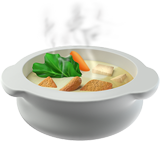
\includegraphics[scale=0.10,natwidth=10,natheight=10]{Pictures/soup.png}}
%\newcommand{\bigsoup}{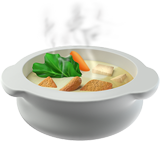
\includegraphics[scale=0.30,natwidth=10,natheight=10]{Pictures/soup.png}}
%\newcommand{\lemon}{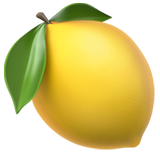
\includegraphics[scale=0.08,natwidth=10,natheight=10]{Pictures/lemon.png}}
%\newcommand{\earth}{
\includegraphics[scale=0.8,natwidth=10,natheight=10]{Pictures/global.png}}
%\newcommand{\local}{
\includegraphics[scale=0.8,natwidth=10,natheight=10]{Pictures/local.png}}
%\newcommand{\biglemon}{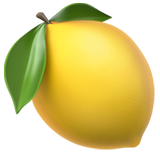
\includegraphics[scale=0.13,natwidth=10,natheight=10]{Pictures/lemon.png}}
%\newcommand{\leaf}{
\includegraphics[scale=0.08,natwidth=10,natheight=10]{Pictures/leaf.png}}
%\newcommand{\sleaf}{
\includegraphics[scale=0.05,natwidth=10,natheight=10]{Pictures/leaf.png}}
%\newcommand{\milk}{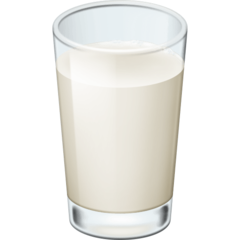
\includegraphics[scale=0.07,natwidth=10,natheight=10]{Pictures/milk.png}}
%\newcommand{\coffee}{
\includegraphics[scale=0.10,natwidth=10,natheight=10]{Pictures/coffee.png}}
%\newcommand{\carrot}{
\includegraphics[scale=0.11,natwidth=10,natheight=10]{Pictures/carrot.png}}
%\newcommand{\bigcarrot}{
\includegraphics[scale=0.15,natwidth=10,natheight=10]{Pictures/carrot.png}}
%\newcommand{\cola}{
\includegraphics[scale=0.08,natwidth=10,natheight=10]{Pictures/cola.png}}
%\newcommand{\scola}{
\includegraphics[scale=0.05,natwidth=10,natheight=10]{Pictures/cola.png}}
%\newcommand{\tea}{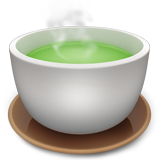
\includegraphics[scale=0.08,natwidth=10,natheight=10]{Pictures/tea.png}}
%\newcommand{\stea}{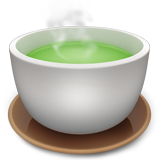
\includegraphics[scale=0.05,natwidth=10,natheight=10]{Pictures/tea.png}}
%\newcommand{\teaa}{
\includegraphics[scale=0.03,natwidth=10,natheight=10]{Pictures/teaaa.jpg}}
%\newcommand{\cow}{
\includegraphics[scale=0.08,natwidth=10,natheight=10]{Pictures/cow.png}}
%\newcommand{\orange}{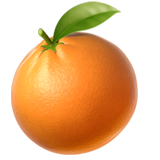
\includegraphics[scale=0.09,natwidth=10,natheight=10]{Pictures/orange.png}}
%\newcommand{\bento}{
\includegraphics[scale=0.09,natwidth=10,natheight=10]{Pictures/bento.png}}
%\newcommand{\sbento}{
\includegraphics[scale=0.06,natwidth=10,natheight=10]{Pictures/bento.png}}
%\newcommand{\bigbento}{
\includegraphics[scale=0.13,natwidth=10,natheight=10]{Pictures/bento.png}}
%\newcommand{\money}{
\includegraphics[scale=0.09,natwidth=10,natheight=10]{Pictures/money.png}}
%\newcommand{\no}{
\includegraphics[scale=0.13,natwidth=10,natheight=10]{Pictures/no.png}}
%\newcommand{\think}{
\includegraphics[scale=0.13,natwidth=10,natheight=10]{Pictures/think.png}}
%\newcommand{\question}{
\includegraphics[scale=0.13,natwidth=10,natheight=10]{Pictures/question.png}}
%\newcommand{\tear}{
\includegraphics[scale=0.13,natwidth=10,natheight=10]{Pictures/tear.png}}
%\newcommand{\infinity}{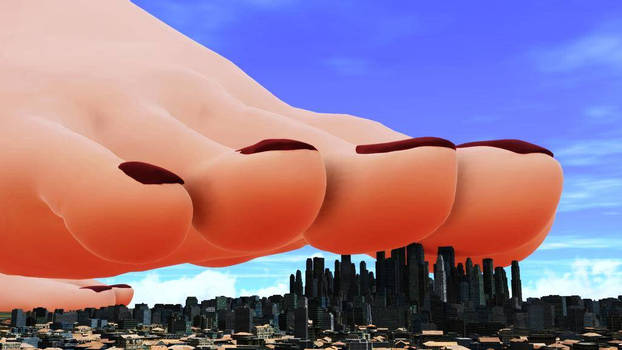
\includegraphics[scale=0.7,natwidth=10,natheight=10]{Pictures/infinity.jpg}}
%\newcommand{\normal}{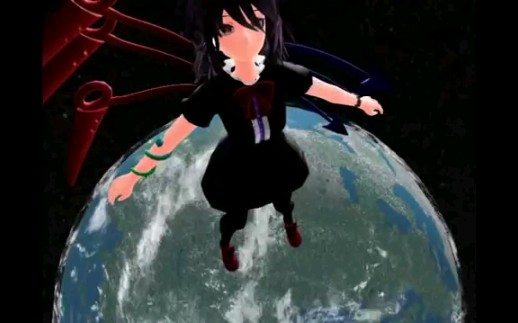
\includegraphics[scale=0.7,natwidth=10,natheight=10]{Pictures/normal.jpg}}
%\newcommand{\boss}{
\includegraphics[scale=0.13,natwidth=10,natheight=10]{Pictures/boss.png}}
%\newcommand{\collision}{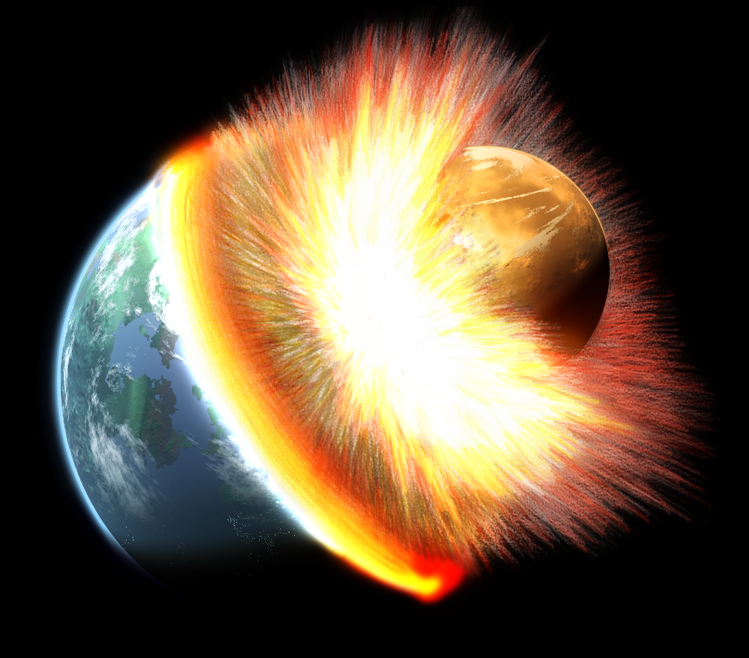
\includegraphics[scale=0.5,natwidth=10,natheight=10]{Pictures/collision.png}}
%\newcommand{\homework}{
\includegraphics[scale=0.13,natwidth=10,natheight=10]{Pictures/homework.png}}
%\newcommand{\sinister}{
\includegraphics[scale=0.13,natwidth=10,natheight=10]{Pictures/sinister.png}}
%\newcommand{\sleep}{
\includegraphics[scale=0.13,natwidth=10,natheight=10]{Pictures/sleep.png}}
%\newcommand{\answer}{
\includegraphics[scale=0.13,natwidth=10,natheight=10]{Pictures/answer.png}}
%\newcommand{\hi}{
\includegraphics[scale=0.13,natwidth=10,natheight=10]{Pictures/hi.png}}
%\newcommand{\spy}{
\includegraphics[scale=0.04,natwidth=10,natheight=10]{Pictures/spy.png}}
%\newcommand{\police}{
\includegraphics[scale=0.2,natwidth=10,natheight=10]{Pictures/police.png}}
%\newcommand{\case}{
\includegraphics[scale=0.1,natwidth=10,natheight=10]{Pictures/box.png}}
%\newcommand{\remote}{
\includegraphics[scale=0.05,natwidth=10,natheight=10]{Pictures/remote.png}}
%\newcommand{\wifi}{
\includegraphics[scale=0.05,natwidth=10,natheight=10]{Pictures/wifi.png}}
%\newcommand{\man}{
\includegraphics[scale=0.1,natwidth=10,natheight=10]{Pictures/man.png}}
%\newcommand{\bow}{
\includegraphics[scale=0.08,natwidth=10,natheight=10]{Pictures/bow.jpg}}
%\newcommand{\house}{
\includegraphics[scale=0.13,natwidth=10,natheight=10]{Pictures/house.png}}
%\newcommand{\convey}{\includegraphics[scale=0.13,natwidth=10,natheight=10]{Pictures/convey.jpg}}

%%%%%%%%%%%%%%%% The above are for pictures %%%%%%%%%%%%%%%%%%%%%%
%%%%%%%%%%%%%%%%%%%%%%%%%%%%%%%%%%%%%%%%%%%%%%%%%%%%%%%%%%%%%%%%%

\long\def\[#1]#2{ \begin{#1}#2\end{#1}}
\makeatletter
\def\m{\@tut\@gobble\@tutt}
\def\@tut#1\@tutt#2{
\@ifnextchar,{\@tut #1 & #2\\\expandafter\expandafter\expandafter\@gobble\expandafter\@gobble\@gobble\@tutt}{
\@ifnextchar.{\begin{pmatrix}#1 &#2\end{pmatrix}\@gobble}{\@tut #1 & #2\@tutt}
}
}
\def\bm{\@tuut\@gobble\@tuutt}
\def\@tuut#1\@tuutt#2{
\@ifnextchar,{\@tuut #1 & #2\cr\expandafter\expandafter\expandafter\@gobble\expandafter\@gobble\@gobble\@tuutt}{
\@ifnextchar.{\bordermatrix{#1 &#2\cr}\@gobble}{\@tuut #1 & #2\@tuutt}
}
}
\makeatother

%%%%% The following are command folders
%\input{Command/script}

%\input{Command/infinity}
\newcommand{\n}{{\color{blue}0}}
\newcommand{\w}{{\color{red}\infty}}
\newcommand{\ac}[1]{\qquad (\; \n^{#1} = 0\; )}
\newcommand{\cn}[1]{\cdot\n^{#1}}

%\input{Command/Drawer}


\newcommand\ko[4]{\begin{scope}[scale=0.5,xshift=#1 cm,yshift=#2 cm]
#3#4
\end{scope}}

\newcommand\dback{
% following 后面
\draw[white,fill={rgb:red,5;green,2;yellow,5}] (10,2)--(6,2)--(6,3)--(12,3);
%following 底面
\draw[white,fill={rgb:red,8;green,1;yellow,8}] (2,0)--(6,0)--(10,2)--(6,2)--(2,0);
\draw[black] (10,2)--(6,2)--(2,0);
% following 内左侧面
\draw[white,fill={rgb:red,5;green,3;yellow,1}] (0,0)--(6,3)--(6,2)--(2,0);
}

\newcommand\dfront{

%following 右侧面
\draw[white,fill={rgb:red,5;green,3;yellow,1}] (6,0)--(12,3)--(12,2)--(6,-1)--(6,0);
% Following the 前面
\draw[white, fill={rgb:red,4;green,2;yellow,1}] (0,0)--(6,0)--(6,-1)--(0,-1)--(0,0);
\draw[white,fill=white] (2,-0.3)--(4,-0.3)--(4,-0.4)--(2,-0.4)--(2,-0.3);
}

\newcommand\nb[1]{\node[shape=circle,fill=white,inner sep=0.5pt] at (0,0) {\textcolor{black}{#1}};}
\newcommand\nw[1]{\node[shape=circle,fill=black,inner sep=0.5pt] at (0,0) {\textcolor{white}{#1}};}
\newcommand\nnw[3]{\node[shape=circle,fill=black,inner sep=0.5pt] at (#2,#3) {\textcolor{white}{#1}};}

\newcommand\bo[1]{
\draw[fill=#1]  (0,0)--(2,0)--(4,1)--(2,1)--(0,0)--(0,-0.3)--(2,-0.3)--(4,0.7)--(4,1);
}

\newcommand\boo[2]{
\draw[fill=#1]  (0,0)--(2,0)--(4,1)--(2,1)--(0,0)--(0,-0.3)--(2,-0.3)--(4,0.7)--(4,1);
\node[shape=circle,fill=white,inner sep=0.5pt] at (2,1) {\textcolor{black}{#2}};
}

\newcommand\booo[3]{
\draw[fill=#1]  (0,0)--(2,0)--(4,1)--(2,1)--(0,0)--(0,-0.3)--(2,-0.3)--(4,0.7)--(4,1);
\node[shape=circle,fill=white,inner sep=0.5pt] at (2,1) {\textcolor{black}{#2}};
\node[shape=circle,fill=white,inner sep=0.5pt] at (2.5,1) {\textcolor{black}{#3}};
}

\newcommand\boooo[4]{
\draw[fill=#1]  (0,0)--(2,0)--(4,1)--(2,1)--(0,0)--(0,-0.3)--(2,-0.3)--(4,0.7)--(4,1);
\node[shape=circle,fill=white,inner sep=0.5pt] at (2,1) {\textcolor{black}{#2}};
\node[shape=circle,fill=white,inner sep=0.5pt] at (2.5,1) {\textcolor{black}{#3}};
\node[shape=circle,fill=white,inner sep=0.5pt] at (3,1) {\textcolor{black}{#4}};
}


\newcommand\booooo[5]{
\draw[fill=#1]  (0,0)--(2,0)--(4,1)--(2,1)--(0,0)--(0,-0.3)--(2,-0.3)--(4,0.7)--(4,1);
\node[shape=circle,fill=white,inner sep=0.5pt] at (2,1) {\textcolor{black}{#2}};
\node[shape=circle,fill=white,inner sep=0.5pt] at (2.5,1) {\textcolor{black}{#3}};
\node[shape=circle,fill=white,inner sep=0.5pt] at (3,1) {\textcolor{black}{#4}};
\node[shape=circle,fill=white,inner sep=0.5pt] at (3.5,1) {\textcolor{black}{#5}};
}





\newcommand\bbo[2]{
\draw[fill=#1]  (0,0)--(2,0)--(4,1)--(2,1)--(0,0)--(0,-0.3)--(2,-0.3)--(4,0.7)--(4,1);
\node[shape=circle,fill=black,inner sep=0.5pt] at (1,0.5) {\textcolor{white}{#2}};
}

\newcommand\bboo[3]{
\draw[fill=#1]  (0,0)--(2,0)--(4,1)--(2,1)--(0,0)--(0,-0.3)--(2,-0.3)--(4,0.7)--(4,1);
\node[shape=circle,fill=white,inner sep=0.5pt] at (2,1) {\textcolor{black}{#2}};
\node[shape=circle,fill=black,inner sep=0.5pt] at (1,0.5) {\textcolor{white}{#3}};
}

\newcommand\bbooo[4]{
\draw[fill=#1]  (0,0)--(2,0)--(4,1)--(2,1)--(0,0)--(0,-0.3)--(2,-0.3)--(4,0.7)--(4,1);
\node[shape=circle,fill=white,inner sep=0.5pt] at (2,1) {\textcolor{black}{#2}};
\node[shape=circle,fill=white,inner sep=0.5pt] at (2.5,1) {\textcolor{black}{#3}};
\node[shape=circle,fill=black,inner sep=0.5pt] at (1,0.5) {\textcolor{white}{#4}};
}

\newcommand\bboooo[5]{
\draw[fill=#1]  (0,0)--(2,0)--(4,1)--(2,1)--(0,0)--(0,-0.3)--(2,-0.3)--(4,0.7)--(4,1);
\node[shape=circle,fill=white,inner sep=0.5pt] at (2,1) {\textcolor{black}{#2}};
\node[shape=circle,fill=white,inner sep=0.5pt] at (2.5,1) {\textcolor{black}{#3}};
\node[shape=circle,fill=white,inner sep=0.5pt] at (3,1) {\textcolor{black}{#4}};
\node[shape=circle,fill=black,inner sep=0.5pt] at (1,0.5) {\textcolor{white}{#5}};
}


\newcommand\bbooooo[6]{
\draw[fill=#1]  (0,0)--(2,0)--(4,1)--(2,1)--(0,0)--(0,-0.3)--(2,-0.3)--(4,0.7)--(4,1);
\node[shape=circle,fill=white,inner sep=0.5pt] at (2,1) {\textcolor{black}{#2}};
\node[shape=circle,fill=white,inner sep=0.5pt] at (2.5,1) {\textcolor{black}{#3}};
\node[shape=circle,fill=white,inner sep=0.5pt] at (3,1) {\textcolor{black}{#4}};
\node[shape=circle,fill=white,inner sep=0.5pt] at (3.5,1) {\textcolor{black}{#5}};
\node[shape=circle,fill=black,inner sep=0.5pt] at (1,0.5) {\textcolor{white}{#6}};
}

\newcommand\bbbo[3]{
\draw[fill=#1]  (0,0)--(2,0)--(4,1)--(2,1)--(0,0)--(0,-0.3)--(2,-0.3)--(4,0.7)--(4,1);
\node[shape=circle,fill=black,inner sep=0.5pt] at (1,0.5) {\textcolor{white}{#2}};
\node[shape=circle,fill=black,inner sep=0.5pt] at (1.5,0.5) {\textcolor{white}{#3}};
}

\newcommand\bbboo[4]{
\draw[fill=#1]  (0,0)--(2,0)--(4,1)--(2,1)--(0,0)--(0,-0.3)--(2,-0.3)--(4,0.7)--(4,1);
\node[shape=circle,fill=white,inner sep=0.5pt] at (2,1) {\textcolor{black}{#2}};
\node[shape=circle,fill=black,inner sep=0.5pt] at (1,0.5) {\textcolor{white}{#3}};
\node[shape=circle,fill=black,inner sep=0.5pt] at (1.5,0.5) {\textcolor{white}{#4}};
}

\newcommand\bbbooo[5]{
\draw[fill=#1]  (0,0)--(2,0)--(4,1)--(2,1)--(0,0)--(0,-0.3)--(2,-0.3)--(4,0.7)--(4,1);
\node[shape=circle,fill=white,inner sep=0.5pt] at (2,1) {\textcolor{black}{#2}};
\node[shape=circle,fill=white,inner sep=0.5pt] at (2.5,1) {\textcolor{black}{#3}};
\node[shape=circle,fill=black,inner sep=0.5pt] at (1,0.5) {\textcolor{white}{#4}};
\node[shape=circle,fill=black,inner sep=0.5pt] at (1.5,0.5) {\textcolor{white}{#5}};
}

\newcommand\bbboooo[6]{
\draw[fill=#1]  (0,0)--(2,0)--(4,1)--(2,1)--(0,0)--(0,-0.3)--(2,-0.3)--(4,0.7)--(4,1);
\node[shape=circle,fill=white,inner sep=0.5pt] at (2,1) {\textcolor{black}{#2}};
\node[shape=circle,fill=white,inner sep=0.5pt] at (2.5,1) {\textcolor{black}{#3}};
\node[shape=circle,fill=white,inner sep=0.5pt] at (3,1) {\textcolor{black}{#4}};
\node[shape=circle,fill=black,inner sep=0.5pt] at (1,0.5) {\textcolor{white}{#5}};
\node[shape=circle,fill=black,inner sep=0.5pt] at (1.5,0.5) {\textcolor{white}{#6}};
}


\newcommand\bbbooooo[7]{
\draw[fill=#1]  (0,0)--(2,0)--(4,1)--(2,1)--(0,0)--(0,-0.3)--(2,-0.3)--(4,0.7)--(4,1);
\node[shape=circle,fill=white,inner sep=0.5pt] at (2,1) {\textcolor{black}{#2}};
\node[shape=circle,fill=white,inner sep=0.5pt] at (2.5,1) {\textcolor{black}{#3}};
\node[shape=circle,fill=white,inner sep=0.5pt] at (3,1) {\textcolor{black}{#4}};
\node[shape=circle,fill=white,inner sep=0.5pt] at (3.5,1) {\textcolor{black}{#5}};
\node[shape=circle,fill=black,inner sep=0.5pt] at (1,0.5) {\textcolor{white}{#6}};
\node[shape=circle,fill=black,inner sep=0.5pt] at (1.5,0.5) {\textcolor{white}{#7}};
}

%\input{Command/ProofControl}
\newif\ift\ttrue
\newif\ifs\strue
\newif\ifi\itrue
\newcommand{\ii}{\ifi}
\newcommand{\iii}{\fi}
\newcommand{\tp}{\ift \textbf{Proof:}}
\newcommand{\app}{\ift \textbf{Standard Proof:}}
\newcommand{\pppp}{\a\aa\textbf{Proof continue }}
\newcommand{\pt}{\fi$\blacksquare$}
\newcommand{\ppa}{\fi$\blacksquare$}
%\input{Command/Tags}
\newcommand*\circled[1]{\tikz[baseline=(char.base)]{
            \node[shape=circle,fill,inner sep=2pt] (char) {\textcolor{white}{#1}};}}
\newcommand*\bl[1]{\tikz[baseline=(char.base)]{
            \node[shape=circle,fill,inner sep=2pt] (char) {\textcolor{white}{#1}};}}
\newcommand*\wh[1]{\tikz[baseline=(char.base)]{
            \node[shape=circle,draw,inner sep=2pt] (char) {#1};}}
%\input{Command/Classify}
\newcommand{\classify}[1]{\fbox{\footnotesize{}$#1$}}
\newcommand{\LI}{{\color{red}\classify{L_I}}}
\newcommand{\II}{{\color{red}\classify{I}}}
\newcommand{\CI}{{\color{red}\classify{C_I}}}
\newcommand{\DI}{{\color{red}\classify{D_I}}}
\newcommand{\NI}{{\color{red}\classify{N_I}}}
\newcommand{\RI}{{\color{red}\classify{R_I}}}
\newcommand{\LS}{{\color{blue}\classify{L_S}}}
\renewcommand{\SS}{{\color{blue}\classify{S}}}
\newcommand{\CS}{{\color{blue}\classify{C_S}}}
\newcommand{\DS}{{\color{blue}\classify{D_S}}}
\newcommand{\NS}{{\color{blue}\classify{N_S}}}
\newcommand{\RS}{{\color{blue}\classify{R_S}}}
%\input{Command/Conveyor}
\pgfmathsetmacro\stack{0}
\def\levelup{\elevate1}%Defalt Value
\def\elevate#1{\pgfmathsetmacro\stack{\stack+1.2*#1}}
\def\su#1{\def\elevate##1{\pgfmathsetmacro\stack{\stack+#1*##1}}}


\pgfmathsetmacro\LeftShift{0}
\pgfmathsetmacro\LeftBox{0}
\def\sb#1{\pgfmathsetmacro\LeftBox{\LeftShift+1.5*#1}}
\def\sf#1{\pgfmathsetmacro\LeftShift{\LeftShift+1.5*#1}}%Defalt Value

\def\B#1{
\abox0\stack{#1}
\levelup
}
\def\BB#1#2{
\abox0\stack{#1}\abox1\stack{#2}
\levelup
}
\def\BBB#1#2#3{
\abox0\stack{#1}\abox1\stack{#2}\abox2\stack{#3}
\levelup
}
\def\BBBB#1#2#3#4{
\abox0\stack{#1}\abox1\stack{#2}\abox2\stack{#3}\abox3\stack{#4}
\levelup
}
\def\BBBBB#1#2#3#4#5{
\abox0\stack{#1}\abox1\stack{#2}\abox2\stack{#3}\abox3\stack{#4}\abox4\stack{#5}
\levelup
}

\def\setgearlevel{\pgfmathsetmacro\gearlevel{\stack-0.1}}

\def\g#1{\setgearlevel
\agear0\gearlevel{#1}\track0\gearlevel0}



\def\gg#1#2{\setgearlevel
\agear0\gearlevel{#1}
\agear1\gearlevel{#2}
\track0\gearlevel1}

\def\ggg#1#2#3{\setgearlevel
\agear0\gearlevel{#1}
\agear1\gearlevel{#2}
\agear2\gearlevel{#3}
\track0\gearlevel2}

\def\gggg#1#2#3#4{\setgearlevel
\agear0\gearlevel{#1}
\agear1\gearlevel{#2}
\agear2\gearlevel{#3}
\agear3\gearlevel{#4}
\track0\gearlevel3}

\def\ggggg#1#2#3#4#5{\setgearlevel
\agear0\gearlevel{#1}
\agear1\gearlevel{#2}
\agear2\gearlevel{#3}
\agear3\gearlevel{#4}
\agear4\gearlevel{#5}
\track0\gearlevel4}

\def\gggggg#1#2#3#4#5#6{\setgearlevel
\agear0\gearlevel{#1}
\agear1\gearlevel{#2}
\agear2\gearlevel{#3}
\agear3\gearlevel{#4}
\agear4\gearlevel{#5}
\agear5\gearlevel{#6}
\track0\gearlevel5}

\def\ggggggg#1#2#3#4#5#6#7{\setgearlevel
\agear0\gearlevel{#1}
\agear1\gearlevel{#2}
\agear2\gearlevel{#3}
\agear3\gearlevel{#4}
\agear4\gearlevel{#5}
\agear5\gearlevel{#6}
\agear6\gearlevel{#7}
\track0\gearlevel6}

\def\gggggggg#1#2#3#4#5#6#7#8{\setgearlevel
\agear0\gearlevel{#1}
\agear1\gearlevel{#2}
\agear2\gearlevel{#3}
\agear3\gearlevel{#4}
\agear4\gearlevel{#5}
\agear5\gearlevel{#6}
\agear6\gearlevel{#7}
\agear7\gearlevel{#8}
\track0\gearlevel7}

\def\ggggggggg#1#2#3#4#5#6#7#8#9{\setgearlevel
\agear0\gearlevel{#1}
\agear1\gearlevel{#2}
\agear2\gearlevel{#3}
\agear3\gearlevel{#4}
\agear4\gearlevel{#5}
\agear5\gearlevel{#6}
\agear6\gearlevel{#7}
\agear7\gearlevel{#8}
\agear8\gearlevel{#9}
\track0\gearlevel8}





\def\abox#1#2#3{%#1=Left position, #2=Top position, #3= Node
    \pgfmathsetmacro\w{#1*1.5}
    \pgfmathsetmacro\p{#2}
    \fill[xshift=-0.5 cm,xshift=\LeftBox cm,yshift=.5cm,rounded corners,red] (\w,\p) node[ultra thick,white,minimum size=12pt] at (\w+0.5,\p+0.5) {\Large #3} rectangle (\w+1,\p+1) ;
}
\def\bbox#1#2#3{%#1=Left position, #2=Top position, #3= Node
    \pgfmathsetmacro\w{#1*1.5}
    \pgfmathsetmacro\p{#2}
    \fill[xshift=-0.5 cm,xshift=\LeftBox cm,yshift=.5cm,rounded corners,fill=pur] (\w,\p) node[ultra thick,white,minimum size=12pt] at (\w+0.5,\p+0.5) {\Large #3} rectangle (\w+1,\p+1) ;
}
\def\cbox#1#2#3{%#1=Left position, #2=Top position, #3= Node
    \pgfmathsetmacro\w{#1*1.5}
    \pgfmathsetmacro\p{#2}
    \fill[xshift=-0.5 cm,xshift=\LeftBox cm,yshift=.5cm,rounded corners,blue] (\w,\p) node[ultra thick,white,minimum size=12pt] at (\w+0.5,\p+0.5) {\Large #3} rectangle (\w+1,\p+1) ;
}
\def\aB#1#2{
\elevate{-1}
\abox#1\stack{#2}
\levelup
}

\def\bB#1#2{
\elevate{-1}
\bbox#1\stack{#2}
\levelup
}
\def\cB#1#2{
\elevate{-1}
\cbox#1\stack{#2}
\levelup
}




\def\track#1#2#3{%This is a track over the gear
\pgfmathsetmacro\w{#1*1.5}
\pgfmathsetmacro\p{#2}
\pgfmathsetmacro\sha{#3*1.5}
\draw[ultra thick,xshift=\w+\LeftShift cm, yshift=\p cm] (0,.5) -- (\sha,.5) arc(90:-90:.5) -- (0,-.5) arc(-90:-270:.5);
\draw[->, thick,blue,xshift=\w+\LeftShift cm, yshift=\p cm] (1,-.7)--(0,-.7) arc(270:90:.7);
\sb0
}


\def\agear#1#2#3{%#1=Left position, #2=Top position, #3= Node
 \pgfmathsetmacro\n{10}%齿轮旋转的角度
    \def\sawtooth{8}
    \pgfmathsetmacro\w{#1*1.5+\LeftShift}
    \pgfmathsetmacro\p{#2}
    \foreach \m in {0,1,...,\sawtooth}
        {\pgfmathsetmacro\x{\m*360/\sawtooth}
         \fill (\w,\p) -- ([xshift=\w cm,yshift=\p cm]\x+\n:.5) arc(\x+\n:\x+\n+20:.5) -- cycle;
    }%这是齿部分
        \fill (\w,\p) circle(.4) node[ultra thick,white,minimum size=12pt] at (\w,\p) { #3};
}

\def\anode#1#2{
    \node[ultra thick,white,minimum size=12pt] at (#1,0) {\Large #2};
}

\def\boxes#1{
    \pgfmathsetmacro\sha{#1-1}
    \foreach \k in {0,...,\sha}{\abox\k0{2}}
}
%\input{Command/Tableau}
\newcommand{\nl}[2]{\dim\left(\ker(#1^{#2})\right)}
\newcommand{\td}{
{Tableau Direction} 

\[zzz]{\B{$\ww$}\B{$\vv$}}
:$\ww=T\vv$
}
\newcommand{\TD}{
{\bf \text{Tableau Direction }}
\ytableaushort{\ww\vv}:$\ww=T\vv$
}
\newcommand{\TDD}[1]{
{\bf \text{Tableau Direction }}

\ytableaushort{\ww\vv}:$\ww=#1\vv$
}

\newcommand{\yt}{\ytableaushort}
\newcommand{\yd}{\ydiagram}
\newcommand{\ys}{\ytableausetup{mathmode, boxsize=1em}}
\newcommand{\ym}{\ytableausetup{mathmode, boxsize=1.5em}}
\newcommand{\yl}{\ytableausetup{mathmode, boxsize=2.5em}}
\newcommand{\yll}{\ytableausetup{mathmode, boxsize=4.5em}}
%\input{Command/convenient}
\newcommand{\mogui}{\vfill{\small\color{gray}\exe Prove this without using \idu\lt.}}
\newcommand\nothing[1]{#1}
%\input{Command/AdjointOperators}
\newcommand{\ttvw}{$\map{T^*}WV$ }
\newcommand{\ssvw}{$\map{S^*}WV$ }
\newcommand{\tvw}{$\map TVW$ }
\newcommand{\svw}{$\map SVW$ }
\newcommand{\swu}{$\map SWU$}
\newcommand{\tvv}{$\map TVV$ }
\newcommand{\vV}{$\vv\in V$ }
\newcommand{\wW}{$\ww\in W$ }
\newcommand{\uU}{$\uu\in U$ }
\newcommand{\adj}{^*}
\newcommand{\pr}[1]{\mathrm{Proj}_{#1}}
\newcommand{\oc}{^\perp}

%\input{Command/Terminology}
\newcommand{\eve}{eigenvector }
\newcommand{\nmo}{normal operator }
\newcommand{\ebas}{eigenbasis }
\newcommand{\oebas}{orthonormal eigenbasis }
\newcommand{\sa}{Self adjoint }
\newcommand{\ut}{unitary }
\newcommand{\op}{Othogonal projection }
\newcommand{\pro}{\textbf{Proof}}
\newcommand{\zs}{\{\0\}}

\newcommand{\idu}{ induced }
\newcommand{\lcb}{ linear combination }

\newcommand{\ldr}{ linear dependence relation }
%\input{Command/Interval}
\newcommand{\qj}[3]{#2<#1<#3}
%\input{Command/index}
\newcommand\nata[3]{L_{\nota{#1}{#2}{#3}}}
%\input{Command/forsome}
\newcommand{\forsome}[2]{
	\qquad \text{for some }#1_1,\cdots,#1_#2\in F
	}
%\vfill

% The following is for Calculus teaching
%The following is for problem making
\newcommand{\baspoly}{ $\{1,x,x^2\}$ is a basis for $V$ }
\newcommand{\polypro}[1]{Let $V=\lPP xabc$, $\map TVV$ is a linear operator defined by $T[f](x)=#1$ }
\newcommand{\polyprot}[1]{Let $V=\lPP xabc$, $W=\lPP tabc$, $\map TVW$ is a linear map defined by $T:f(x)\mapsto #1$ }

\newcommand{\nota}[3]{\left[#1\right]_{#2}^{#3}}
\newcommand{\notaw}[3]{\left[#1\right]^{#2}_{#3}}





%The following is for polynomial notations
\newcommand{\Field}{F}
\newcommand{\lPP}[4]{P_{2,#1}=\{#2#1^2+#3#1+#4,\text{ where }#2,#3,#4\in \Field\}}
\newcommand{\lP}[3]{P_{1,#1}=\{#2#1+#3,\text{ where }#2,#3\in \Field\}}
\newcommand{\lPPP}[5]{P_{3,#1}=\{#2#1^3+#3#1^2+#4#1+#5,\text{ where }#2,#3,#4,#5\in \Field\}}
\newcommand{\f}{\mathrm{F}}
% The following is for existence uniqueness argument
\newcommand{\ch}{\mathrm{char}}
\newcommand{\ce}{{\mathcal E}}
\newcommand{\cw}{{\mathcal F}}
\newcommand{\cv}{{\mathcal G}}
\newcommand{\cd}{{\mathcal H}}
\newcommand{\be}[1]{\mathcal{E}=\basis \ee#1}
\newcommand{\bw}[1]{\mathcal{F}=\basis \ww#1}
\newcommand{\bv}[1]{\mathcal{G}=\basis \vv#1}
\newcommand{\bd}[1]{\mathcal{H}=\basis{\vec d}#1}
\newcommand{\uu}{\vec{u}}
\newcommand{\obe}[1]{\obasis \ee#1}
\newcommand{\obw}[1]{\obasis \ww#1}
\newcommand{\obv}[1]{\obasis \vv#1}
\newcommand{\obd}[1]{\obasis{\vec d}#1}
\definecolor{pur}{RGB}{255,0,255}

\newcommand{\spa}{\textbf{ span }}
\newcommand{\spab}{\textbf{ spanned by }}


\newcommand{\bn}{\textbf{\color{blue} Numerical Property }}
\newcommand{\sws}{\textbf{\color{blue} span the whole space }}
%\newcommand{\sws}{\textbf{\color{blue} 张满全空间 }}
\newcommand{\swss}{\textbf{\color{blue} span the whole subspace }}
\newcommand{\te}{\textbf{\color{blue} there exists }}
\newcommand{\ifu}{\textbf{\color{blue} but may not unique }}
\newcommand{\stws}{\textbf{\color{blue} sum to the whole space }}



\newcommand{\SI}{{\color{blue}\classify{{\color{blue}S}\mapsto{\color{red}I}}}}
\newcommand{\IS}{{\color{red}\classify{{\color{red}I}\mapsto{\color{blue}S}}}}

\newcommand{\exce}{\textbf{\color{blue} existence }}
\newcommand{\scy}{\textbf{\color{blue} sufficiency }}
%\newcommand{\exce}{\textbf{\color{blue} 存在性 }}
\newcommand{\enu}{\textbf{\color{blue} constructive language }}
%\newcommand{\enu}{\textbf{\color{blue} 枚举性语言}}
\newcommand{\enuv}{\textbf{\color{blue} constructive} }
%\newcommand{\enuv}{\textbf{\color{blue} 枚举性的}}

\newcommand{\leasto}{\textbf{\color{blue} at least one }}
%\newcommand{\leasto}{\textbf{\color{blue} 至少有一个 }}
\newcommand{\exi}{\textbf{\color{blue} exists }}
%\newcommand{\exi}{\textbf{\color{blue} 存在 }}
\newcommand{\more}{\textbf{\color{blue} no less than }}
\newcommand{\nored}{\textbf{\color{blue} independent equations }}
\newcommand{\exx}{\textbf{\color{blue} 有 }}
\newcommand{\excp}{\textbf{\color{blue} existence problem }}
\newcommand{\rc}{\textbf{\color{blue} right cancellation }}
%\newcommand{\rc}{\textbf{\color{blue} 可右消去}}
\newcommand{\rf}{\textbf{\color{blue} right factor }}
%\newcommand{\rf}{\textbf{\color{blue} 右因子 }}
\newcommand{\riv}{\textbf{\color{blue} right inverse }}


\newcommand{\sub}{\textbf{\color{blue} sub}}


\newcommand{\sur}{\textbf{\color{blue} surjective }}
%\newcommand{\sur}{\textbf{\color{blue} 满射 }}
\newcommand{\pa}{\textbf{\color{blue} parameters }}
%\newcommand{\pa}{\textbf{\color{blue}参数}}
\newcommand{\pation}{\textbf{\color{black} parametrization }}

\newcommand{\img}{\textbf{\color{black} image }}

\newcommand{\rn}{\textbf{\color{red} Numerical Property }}
\newcommand{\des}{\textbf{\color{red} descriptive language }}
%\newcommand{\des}{\textbf{\color{red} 概括性语言}}
\newcommand{\desv}{\textbf{\color{red} descriptive }}
%\newcommand{\desv}{\textbf{\color{red} 概括性的}}

\newcommand{\unce}{\textbf{\color{red} uniqueness }}
%\newcommand{\unce}{\textbf{\color{red} 唯一性 }}
\newcommand{\ecy}{\textbf{\color{red} ecnomical }}
\newcommand{\mosto}{\textbf{\color{red} at most one }}
%\newcommand{\mosto}{\textbf{\color{red} 至多有一个 }}
\newcommand{\less}{\textbf{\color{red} no more than }}
\newcommand{\ife}{\textbf{\color{red} if there exists }}
\newcommand{\un}{\textbf{\color{red} unique }}
\newcommand{\uny}{\textbf{\color{red} uniquely }}
\newcommand{\nofree}{\textbf{\color{red} no free variables }}
%\newcommand{\un}{\textbf{\color{red} 唯一 }}
\newcommand{\unp}{\textbf{\color{red} uniqueness problem }}
\newcommand{\lc}{\textbf{\color{red} left cancellation }}
%\newcommand{\lc}{\textbf{\color{red} 可左消去 }}
\newcommand{\lf}{\textbf{\color{red} left factor }}
%\newcommand{\lf}{\textbf{\color{red} 左因子 }}
\newcommand{\liv}{\textbf{\color{red} left inverse }}

\newcommand{\quo}{\textbf{\color{red} quotient}}

\newcommand{\inj}{\textbf{\color{red} injective }}
%\newcommand{\inj}{\textbf{\color{red} 单射 }}
\newcommand{\cla}{\textbf{\color{red}class }}
\newcommand{\cl}{\textbf{\color{red}property }}
%\newcommand{\cla}{\textbf{\color{red}类别}}
\newcommand{\clation}{\textbf{\color{black}classification}}
\newcommand{\li}{\textbf{\color{red} linealy independent }}
%\newcommand{\li}{\textbf{\color{red} 线性独立 }}
\newcommand{\ids}{\textbf{\color{red} is a direct sum }}


\newcommand{\pimg}{\textbf{\color{black} preimage }}
\newcommand{\kn}{\textbf{\color{red} kernel }}

\newcommand{\iso}{\textbf{\color{pur} isomorphism }}
%\newcommand{\iso}{\textbf{\color{pur} 双射 }}
\newcommand{\teun}{\textbf{\color{pur} there exists an unique }}
%\newcommand{\teun}{\textbf{\color{pur} 存在唯一 }}
\newcommand{\eeun}{\textbf{\color{pur} 唯一指定 }}
\newcommand{\exacto}{\textbf{\color{pur} exactly one }}
%\newcommand{\exacto}{\textbf{\color{pur} 恰好有一个 }}
\newcommand{\bas}{\textbf{\color{pur} basis }}
%\newcommand{\bas}{\textbf{\color{pur} 基 }}
\newcommand{\dstws}{\textbf{\color{pur} direct sum to the whole space }}
\newcommand{\dst}{\textbf{\color{pur} direct sum decomposition }}
\newcommand{\inve}{\textbf{\color{pur} invertible }}
\newcommand{\same}{\textbf{\color{pur} is the same as }}
%\newcommand{\inve}{\textbf{\color{pur} 可逆 }}
\newcommand{\pn}{\textbf{\color{pur} Numerical Property }}
\newcommand{\np}{\textbf{\color{pur} No Problem }}

\newcommand{\lt}{linear transformation }
\newcommand{\lo}{linear operator }
\newcommand{\rs}{restriction }
\newcommand{\sus}{subspace }
\newcommand{\insus}{invariant subspace }
\newcommand{\ges}{generalized eigenspace }
\newcommand{\ev}{eigenvalue }
\newcommand{\cp}{characteristic polynomial }

% The following is for pictures

\newcommand{\bb}{\x}
\newcommand{\apple}{\includegraphics[scale=0.08,natwidth=10,natheight=10]{Pictures/apple.png}}
\newcommand{\bigapple}{\includegraphics[scale=0.13,natwidth=10,natheight=10]{Pictures/apple.png}}
\newcommand{\peach}{\includegraphics[scale=0.08,natwidth=10,natheight=10]{Pictures/peach.png}}
\newcommand{\bigpeach}{\includegraphics[scale=0.13,natwidth=10,natheight=10]{Pictures/peach.png}}
\newcommand{\bean}{\includegraphics[scale=0.07,natwidth=10,natheight=10]{Pictures/bean.png}}
\newcommand{\sbean}{\includegraphics[scale=0.04,natwidth=10,natheight=10]{Pictures/bean.png}}
\newcommand{\soup}{\includegraphics[scale=0.10,natwidth=10,natheight=10]{Pictures/soup.png}}
\newcommand{\ssoup}{\includegraphics[scale=0.07,natwidth=10,natheight=10]{Pictures/soup.png}}
\newcommand{\bigsoup}{\includegraphics[scale=0.30,natwidth=10,natheight=10]{Pictures/soup.png}}
\newcommand{\lemon}{\includegraphics[scale=0.08,natwidth=10,natheight=10]{Pictures/lemon.png}}
\newcommand{\slemon}{\includegraphics[scale=0.05,natwidth=10,natheight=10]{Pictures/lemon.png}}
\newcommand{\biglemon}{\includegraphics[scale=0.13,natwidth=10,natheight=10]{Pictures/lemon.png}}
\newcommand{\leaf}{\includegraphics[scale=0.08,natwidth=10,natheight=10]{Pictures/leaf.png}}
\newcommand{\sleaf}{\includegraphics[scale=0.05,natwidth=10,natheight=10]{Pictures/leaf.png}}
\newcommand{\milk}{\includegraphics[scale=0.07,natwidth=10,natheight=10]{Pictures/milk.png}}
\newcommand{\smilk}{\includegraphics[scale=0.04,natwidth=10,natheight=10]{Pictures/milk.png}}
\newcommand{\coffee}{\includegraphics[scale=0.10,natwidth=10,natheight=10]{Pictures/coffee.png}}
\newcommand{\scoffee}{\includegraphics[scale=0.07,natwidth=10,natheight=10]{Pictures/coffee.png}}
\newcommand{\carrot}{\includegraphics[scale=0.11,natwidth=10,natheight=10]{Pictures/carrot.png}}
\newcommand{\bigcarrot}{\includegraphics[scale=0.15,natwidth=10,natheight=10]{Pictures/carrot.png}}
\newcommand{\cola}{\includegraphics[scale=0.08,natwidth=10,natheight=10]{Pictures/cola.png}}
\newcommand{\scola}{\includegraphics[scale=0.05,natwidth=10,natheight=10]{Pictures/cola.png}}
\newcommand{\tea}{\includegraphics[scale=0.08,natwidth=10,natheight=10]{Pictures/tea.png}}
\newcommand{\stea}{\includegraphics[scale=0.05,natwidth=10,natheight=10]{Pictures/tea.png}}
\newcommand{\teaa}{\includegraphics[scale=0.03,natwidth=10,natheight=10]{Pictures/teaaa.jpg}}
\newcommand{\cow}{\includegraphics[scale=0.08,natwidth=10,natheight=10]{Pictures/cow.png}}
\newcommand{\orange}{\includegraphics[scale=0.09,natwidth=10,natheight=10]{Pictures/orange.png}}
\newcommand{\bento}{\includegraphics[scale=0.09,natwidth=10,natheight=10]{Pictures/bento.png}}
\newcommand{\sbento}{\includegraphics[scale=0.04,natwidth=10,natheight=10]{Pictures/bento.png}}
\newcommand{\bigbento}{\includegraphics[scale=0.13,natwidth=10,natheight=10]{Pictures/bento.png}}
\newcommand{\money}{\includegraphics[scale=0.09,natwidth=10,natheight=10]{Pictures/money.png}}
\newcommand{\buxie}{\includegraphics[scale=0.05,natwidth=10,natheight=10]{Pictures/buxie.png}}
\newcommand{\no}{\includegraphics[scale=0.13,natwidth=10,natheight=10]{Pictures/no.png}}
\newcommand{\think}{\includegraphics[scale=0.13,natwidth=10,natheight=10]{Pictures/think.png}}
\newcommand{\question}{\includegraphics[scale=0.13,natwidth=10,natheight=10]{Pictures/question.png}}
\newcommand{\tear}{\includegraphics[scale=0.13,natwidth=10,natheight=10]{Pictures/tear.png}}
\newcommand{\boss}{\includegraphics[scale=0.13,natwidth=10,natheight=10]{Pictures/boss.png}}
\newcommand{\homework}{\includegraphics[scale=0.13,natwidth=10,natheight=10]{Pictures/homework.png}}
\newcommand{\sinister}{\includegraphics[scale=0.13,natwidth=10,natheight=10]{Pictures/sinister.png}}
\newcommand{\sleep}{\includegraphics[scale=0.13,natwidth=10,natheight=10]{Pictures/sleep.png}}
\newcommand{\answer}{\includegraphics[scale=0.13,natwidth=10,natheight=10]{Pictures/answer.png}}
\newcommand{\hi}{\includegraphics[scale=0.6,natwidth=10,natheight=10]{Pictures/hi.png}}
\newcommand{\spy}{\includegraphics[scale=0.04,natwidth=10,natheight=10]{Pictures/spy.png}}
\newcommand{\police}{\includegraphics[scale=0.2,natwidth=10,natheight=10]{Pictures/police.png}}
\newcommand{\case}{\includegraphics[scale=0.1,natwidth=10,natheight=10]{Pictures/box.png}}
\newcommand{\remote}{\includegraphics[scale=0.05,natwidth=10,natheight=10]{Pictures/remote.png}}
\newcommand{\wifi}{\includegraphics[scale=0.05,natwidth=10,natheight=10]{Pictures/wifi.png}}
\newcommand{\man}{\includegraphics[scale=0.1,natwidth=10,natheight=10]{Pictures/man.png}}
\newcommand{\bow}{\includegraphics[scale=0.08,natwidth=10,natheight=10]{Pictures/bow.jpg}}
\newcommand{\house}{\includegraphics[scale=0.13,natwidth=10,natheight=10]{Pictures/house.png}}
\newcommand{\convey}{\includegraphics[scale=0.13,natwidth=10,natheight=10]{Pictures/convey.jpg}}
\newcommand{\drawer}{\includegraphics[scale=0.13,natwidth=10,natheight=10]{Pictures/drawer.png}}
\newcommand{\book}{\includegraphics[scale=0.13,natwidth=10,natheight=10]{Pictures/book.png}}
\newcommand{\rbook}{\includegraphics[scale=0.013,natwidth=10,natheight=10]{Pictures/redbook.png}}
\newcommand{\bbook}{\includegraphics[scale=0.013,natwidth=10,natheight=10]{Pictures/bluebook.png}}

\newcommand{\h}{\cellcolor{red!50}}
\newcommand{\y}{\cellcolor{yellow!50}}
\newcommand{\e}{\cellcolor{blue!50}}



\newenvironment{s}{\begin{scope}}{\end{scope}}
\renewcommand{\1}{\textcircled{1}}
\newcommand{\C}{\tikz\draw[red,fill=red] (0,0) circle (.9ex);}
\newcommand{\CCC}{\tikz\draw[blue,fill=blue] (0,0) circle (.9ex);}
\newcommand{\CCCC}{\tikz\draw[cyan,fill=cyan] (0,0) circle (.9ex);}
%\newcommand{\red}[1]{{\color{red}{#1}}}





\newcommand{\spann}{\mathrm{span}}
\newcommand{\comp}{\mathrm{comp}}
\newcommand{\proj}{\mathrm{proj}}
%The following is designed for display transformation
\newcommand{\dis}[2]{
\begin{columns}
\column{0.45\textwidth}
#1
\column{0.1\textwidth}
%$\rightarrow$
\column{0.45\textwidth}
#2
\end{columns}
}
%The following are for drawing pictures
\newcommand{\org}{\draw[fill] (0,0) circle[radius=0.1] node[below]{O};}
\newcommand{\wangge}[4]{\draw[gray] (#1,#2) grid (#3,#4);}
\newcommand{\xaxis}[2]{\draw[black,->](#1,0)--(#2,0);}
\newcommand{\yaxis}[2]{\draw[black,->](0,#1)--(0,#2);}
\newcommand{\dasis}[1]{\draw[->,ultra thick](0,0)--(1,0) node[right]{$#1_1$};\draw[->,ultra thick](0,0)--(0,1) node[above]{$#1_2$};}
\newcommand{\asis}[5]{\draw[->,ultra thick,opacity=0.7,red](0,0)--(#2,#3) node[right]{$#1_1$};\draw[->,ultra thick,opacity=0.7,red](0,0)--(#4,#5) node[above]{$#1_2$};}
\newcommand{\basisspace}[1]{\org\wangge{-#1}{-#1}{#1}{#1}\dasis{\ee}}
%The following are some given pictures
\newcommand{\smileface}{
\draw[thick] (0,0) circle[radius=1];
\draw[thick] plot [smooth,tension=1.5] coordinates{(-0.5,-0.5) (0,-0.8) (0.5,-0.5)};
\draw[thick] plot [smooth,tension=1.5] coordinates{(0.2,-0.76) (0.4,-0.3) (0.5,-0.5)};
\draw [thick, fill=black] (0,-0.2) circle (0.1);
\draw[thick] plot [smooth,tension=1.5] coordinates{(-0.4,0.4) (-0.3,0.5) (-0.2,0.4)};
\draw[thick] plot [smooth,tension=1.5] coordinates{(0.4,0.4) (0.3,0.5) (0.2,0.4)};
}
%The following are more advanced package, modified on 11,11,2018
\newcommand{\p}[4][red]{\draw[fill=#1] (#2,#3)circle[radius=0.1] node[right]{$#4$};}
\newcommand{\vve}[6][black]{\draw[->,#1,ultra thick] (#2,#3)--(#2+#4,#3+#5) node[above]{$#6$};}
\newcommand{\ve}[4][black]{\draw[->,#1,ultra thick] (0,0)--(#2,#3) node[above]{$#4$};}
\newcommand{\para}[7][none]{\draw[fill=#1] (#2,#3)--(#2+#4,#3+#5)--(#2+#6+#4,#3+#7+#5)--(#2+#6,#3+#7)--(#2,#3);}
\newcommand{\rec}[5][none]{\para[#1]{#2}{#3}{#4}{0}{0}{#5}}
\renewcommand{\cir}[4][none]{\draw[fill=#1] (#2,#3) circle[radius=#4];}
\newcommand{\grid}[5][help lines]{\foreach \i in {#3,...,#5}
		{\draw[#1](#2-0.5,\i)--(#4+0.5,\i);}
	\foreach \i in {#2,...,#4}
		{\draw[#1](\i,#3-0.5)--(\i,#5+0.5);}
}
\newcommand{\zbx}[1]{\grid{-#1}{-#1}{#1}{#1}\xis{-#1}{-#1}{#1}{#1}}
\newcommand{\xgrid}[2][help lines]{\grid[#1]{-#2}{-#2}{#2}{#2}}
\newcommand{\net}[5][help lines]{\foreach \i in {#3,...,#5}
		{\draw[#1](#2,\i)--(#4,\i);}
	\foreach \i in {#2,...,#4}
		{\draw[#1](\i,#3)--(\i,#5);}
}
\newcommand{\xnet}[2][help lines]{\net[#1]{-#2}{-#2}{#2}{#2}}
\newcommand{\xis}[4]{\draw[black,->](#1-1,0)--(#3+1,0) node[right]{$x$};\draw[black,->](0,#2-1)--(0,#4+1) node[above]{$y$};}
\newcommand{\xxis}[1]{\xis{-#1}{-#1}{#1}{#1}}


%The following command is used for drawing angles

\newcommand{\an}[4]{pic["#1", draw=orange, ->, angle eccentricity=1.2, angle radius=.6cm]
    {angle=#2--#3--#4}}



\long\def\[#1]#2{ \begin{#1}#2\end{#1}}
%The above are more advanced
%\newcommand{\rec}[5][none]{\draw[fill=#1] ()}

\newcommand{\dian}[3][]{\huadian{#2}{#3}{#1}}
\newcommand{\func}[3]{\draw[domain=#1:#2,smooth,variable=\x,blue] plot ({\x},{#3});}
\newcommand{\funcc}[3]{\draw[domain=#1:#2,smooth,variable=\x,blue,thick] plot ({\x},{#3});}
\newcommand{\funccc}[3]{\draw[domain=#1:#2,smooth,variable=\x,blue,ultra thick] plot ({\x},{#3});}
\newcommand{\huadian}[3]{\draw[fill=red] (#1,#2)circle[radius=0.1] node[right]{$#3$};}
\newcommand{\huadiandian}[3]{\draw[fill=blue] (#1,#2)circle[radius=0.1] node[right]{$#3$};}
\newcommand{\vblack}[3]{\draw[->,black,ultra thick] (0,0)--(#1,#2) node[above]{$#3$};}
\newcommand{\vred}[3]{\draw[->,red,ultra thick] (0,0)--(#1,#2) node[above]{$#3$};}
\newcommand{\vpurple}[3]{\draw[->,purple,ultra thick] (0,0)--(#1,#2) node[above]{$#3$};}
\newcommand{\vgreen}[3]{\draw[->,green,ultra thick] (0,0)--(#1,#2) node[above]{$#3$};}
\newcommand{\vblue}[3]{\draw[->,blue,ultra thick] (0,0)--(#1,#2) node[above]{$#3$};}
\newcommand{\rh}[2]{\draw[ultra thick,red] (0.5,0) arc(0:#1:0.5) node[ultra thick,right] {$#2^\circ$};}
\newcommand{\rv}[2]{\draw[ultra thick,red] (0,0.5) arc(90:90+#1:0.5) node[ultra thick,left] {$#2^\circ$};}
\renewcommand{\im}{\mathrm{Im}}
\renewcommand{\Im}{\mathrm{Im}}
\renewcommand{\ker}{\mathrm{Ker}}
\newcommand{\rank}{\mathrm{Rank }  }


\newcommand{\pp}[2]{#1\rr{#2_1}{#2_2}=\rr{#2_1}{#2_2}}
\newcommand{\tpp}[2]{\begin{array}{ll}&#1\rr{#2_1}{#2_2}\\\\=&\rr{#2_1}{#2_2}\end{array}}
\newcommand{\ppp}[2]{#1\rrr{#2_1}{#2_2}{#2_3}=\rrr{#2_1}{#2_2}{#2_3}}
\newcommand{\tppp}[2]{\begin{array}{ll}&#1\rrr{#2_1}{#2_2}{#2_3}\\\\=&\rrr{#2_1}{#2_2}{#2_3}\end{array}}



\newcommand\co[1]{\column{0.#1\textwidth}}
\newcommand{\xequal}[1]{\overset{#1}{=\joinrel=}}
%%% The above are commands

